% Heather burning and cutting on red grouse count areas: report version 2 (internal file name v6).
% Build: report/build.sh (xelatex via latexmk). Figures and tables: python report/make_figures.py
\documentclass[11pt,a4paper]{article}

\newcommand{\reporthead}{Heather management on red grouse count areas}
\newcommand{\reportdate}{Version 2, October 2026}
% Shared style for the heather management reports (report_v6.tex, beetle_report.tex).
% Each report defines \reporthead and \reportdate before % Shared style for the heather management reports (report_v6.tex, beetle_report.tex).
% Each report defines \reporthead and \reportdate before % Shared style for the heather management reports (report_v6.tex, beetle_report.tex).
% Each report defines \reporthead and \reportdate before \input{style}.
% ---------------------------------------------------------------- fonts and language
\usepackage{amsmath}
\usepackage{fontspec}
\usepackage{unicode-math}
\setmainfont{texgyrepagella}[Extension=.otf,UprightFont=*-regular,BoldFont=*-bold,
  ItalicFont=*-italic,BoldItalicFont=*-bolditalic]
\setsansfont{Helvetica Neue}
\setmathfont{texgyrepagella-math.otf}
\usepackage[british]{babel}
\usepackage{microtype}

% ---------------------------------------------------------------- page
\usepackage[a4paper,top=2.5cm,bottom=2.5cm,left=2.4cm,right=2.4cm,headheight=14pt]{geometry}
\setlength{\parskip}{0.55em}
\setlength{\parindent}{0pt}
\linespread{1.06}

\usepackage{xcolor}
\definecolor{accent}{HTML}{1F4E79}
\definecolor{accentlight}{HTML}{EEF3F9}
\definecolor{muted}{HTML}{5F6B7A}
\definecolor{rulegrey}{HTML}{B8C2CC}

\usepackage{fancyhdr}
\pagestyle{fancy}
\fancyhf{}
\fancyhead[L]{\sffamily\footnotesize\color{muted}\reporthead}
\fancyhead[R]{\sffamily\footnotesize\color{muted}\reportdate}
\fancyfoot[C]{\sffamily\footnotesize\thepage}
\renewcommand{\headrulewidth}{0.4pt}
\renewcommand{\headrule}{\hbox to\headwidth{\color{rulegrey}\leaders\hrule height \headrulewidth\hfill}}
\fancypagestyle{plain}{\fancyhf{}\fancyfoot[C]{\sffamily\footnotesize\thepage}\renewcommand{\headrulewidth}{0pt}}

% ---------------------------------------------------------------- headings and contents
\usepackage{titlesec}
\titleformat{\section}{\sffamily\Large\bfseries\color{accent}}{\thesection}{0.7em}{}
\titleformat{\subsection}{\sffamily\large\bfseries\color{accent}}{\thesubsection}{0.6em}{}
\titleformat{\subsubsection}{\sffamily\normalsize\bfseries}{\thesubsubsection}{0.5em}{}
\titlespacing*{\section}{0pt}{1.8em}{0.6em}
\titlespacing*{\subsection}{0pt}{1.3em}{0.4em}
\titlespacing*{\subsubsection}{0pt}{1.0em}{0.2em}

\usepackage{tocloft}
\renewcommand{\cfttoctitlefont}{\sffamily\Large\bfseries\color{accent}}
\renewcommand{\cftsecfont}{\sffamily\bfseries}
\renewcommand{\cftsecpagefont}{\sffamily\bfseries}
\renewcommand{\cftsecleader}{\cftdotfill{\cftdotsep}}
\setlength{\cftbeforesecskip}{0.2em}
\setlength{\cftbeforetoctitleskip}{0pt}
\setlength{\cftaftertoctitleskip}{0.8em}
\renewcommand{\cftsubsecfont}{\small}
\renewcommand{\cftsubsecpagefont}{\small}
\setlength{\cftbeforesubsecskip}{0pt}
\setcounter{tocdepth}{2}

% ---------------------------------------------------------------- floats, tables, lists
\usepackage{graphicx}
\graphicspath{{figures/}}
\usepackage{booktabs,tabularx,array,threeparttable,makecell}
\renewcommand{\arraystretch}{1.18}
\setlength{\aboverulesep}{0.3ex}
\setlength{\belowrulesep}{0.5ex}
\usepackage{caption}
\captionsetup{font=small,labelfont={bf,sf,color=accent},labelsep=period,justification=justified,
  singlelinecheck=false,skip=6pt}
\captionsetup[table]{position=top}
\usepackage{float}
\usepackage[section]{placeins}
\usepackage{needspace}
\usepackage{enumitem}
\setlist{itemsep=0.25em,topsep=0.3em,parsep=0pt,leftmargin=1.3em}
\newcolumntype{L}{>{\raggedright\arraybackslash}X}

% ---------------------------------------------------------------- boxes and diagrams
\usepackage[most]{tcolorbox}
\newtcolorbox{keybox}[1]{enhanced,breakable,colback=accentlight,colframe=accent,boxrule=0.6pt,arc=1.5pt,
  left=9pt,right=9pt,top=7pt,bottom=7pt,fonttitle=\sffamily\bfseries,coltitle=white,title=#1}
\newtcolorbox{notebox}{enhanced,colback=white,colframe=rulegrey,boxrule=0.5pt,arc=1.5pt,
  left=8pt,right=8pt,top=5pt,bottom=5pt}
\usepackage{tikz}
\usetikzlibrary{positioning,arrows.meta}

% ---------------------------------------------------------------- references and links
\usepackage[round,authoryear]{natbib}
\setlength{\bibsep}{0.35em}
\usepackage{hyperref}
\hypersetup{colorlinks=true,linkcolor=accent,citecolor=accent,urlcolor=accent}

\newcommand{\figref}[1]{Figure~\ref{#1}}
\newcommand{\tabref}[1]{Table~\ref{#1}}
\newcommand{\secref}[1]{Section~\ref{#1}}
\newcommand{\appref}[1]{Appendix~\ref{#1}}

.
% ---------------------------------------------------------------- fonts and language
\usepackage{amsmath}
\usepackage{fontspec}
\usepackage{unicode-math}
\setmainfont{texgyrepagella}[Extension=.otf,UprightFont=*-regular,BoldFont=*-bold,
  ItalicFont=*-italic,BoldItalicFont=*-bolditalic]
\setsansfont{Helvetica Neue}
\setmathfont{texgyrepagella-math.otf}
\usepackage[british]{babel}
\usepackage{microtype}

% ---------------------------------------------------------------- page
\usepackage[a4paper,top=2.5cm,bottom=2.5cm,left=2.4cm,right=2.4cm,headheight=14pt]{geometry}
\setlength{\parskip}{0.55em}
\setlength{\parindent}{0pt}
\linespread{1.06}

\usepackage{xcolor}
\definecolor{accent}{HTML}{1F4E79}
\definecolor{accentlight}{HTML}{EEF3F9}
\definecolor{muted}{HTML}{5F6B7A}
\definecolor{rulegrey}{HTML}{B8C2CC}

\usepackage{fancyhdr}
\pagestyle{fancy}
\fancyhf{}
\fancyhead[L]{\sffamily\footnotesize\color{muted}\reporthead}
\fancyhead[R]{\sffamily\footnotesize\color{muted}\reportdate}
\fancyfoot[C]{\sffamily\footnotesize\thepage}
\renewcommand{\headrulewidth}{0.4pt}
\renewcommand{\headrule}{\hbox to\headwidth{\color{rulegrey}\leaders\hrule height \headrulewidth\hfill}}
\fancypagestyle{plain}{\fancyhf{}\fancyfoot[C]{\sffamily\footnotesize\thepage}\renewcommand{\headrulewidth}{0pt}}

% ---------------------------------------------------------------- headings and contents
\usepackage{titlesec}
\titleformat{\section}{\sffamily\Large\bfseries\color{accent}}{\thesection}{0.7em}{}
\titleformat{\subsection}{\sffamily\large\bfseries\color{accent}}{\thesubsection}{0.6em}{}
\titleformat{\subsubsection}{\sffamily\normalsize\bfseries}{\thesubsubsection}{0.5em}{}
\titlespacing*{\section}{0pt}{1.8em}{0.6em}
\titlespacing*{\subsection}{0pt}{1.3em}{0.4em}
\titlespacing*{\subsubsection}{0pt}{1.0em}{0.2em}

\usepackage{tocloft}
\renewcommand{\cfttoctitlefont}{\sffamily\Large\bfseries\color{accent}}
\renewcommand{\cftsecfont}{\sffamily\bfseries}
\renewcommand{\cftsecpagefont}{\sffamily\bfseries}
\renewcommand{\cftsecleader}{\cftdotfill{\cftdotsep}}
\setlength{\cftbeforesecskip}{0.2em}
\setlength{\cftbeforetoctitleskip}{0pt}
\setlength{\cftaftertoctitleskip}{0.8em}
\renewcommand{\cftsubsecfont}{\small}
\renewcommand{\cftsubsecpagefont}{\small}
\setlength{\cftbeforesubsecskip}{0pt}
\setcounter{tocdepth}{2}

% ---------------------------------------------------------------- floats, tables, lists
\usepackage{graphicx}
\graphicspath{{figures/}}
\usepackage{booktabs,tabularx,array,threeparttable,makecell}
\renewcommand{\arraystretch}{1.18}
\setlength{\aboverulesep}{0.3ex}
\setlength{\belowrulesep}{0.5ex}
\usepackage{caption}
\captionsetup{font=small,labelfont={bf,sf,color=accent},labelsep=period,justification=justified,
  singlelinecheck=false,skip=6pt}
\captionsetup[table]{position=top}
\usepackage{float}
\usepackage[section]{placeins}
\usepackage{needspace}
\usepackage{enumitem}
\setlist{itemsep=0.25em,topsep=0.3em,parsep=0pt,leftmargin=1.3em}
\newcolumntype{L}{>{\raggedright\arraybackslash}X}

% ---------------------------------------------------------------- boxes and diagrams
\usepackage[most]{tcolorbox}
\newtcolorbox{keybox}[1]{enhanced,breakable,colback=accentlight,colframe=accent,boxrule=0.6pt,arc=1.5pt,
  left=9pt,right=9pt,top=7pt,bottom=7pt,fonttitle=\sffamily\bfseries,coltitle=white,title=#1}
\newtcolorbox{notebox}{enhanced,colback=white,colframe=rulegrey,boxrule=0.5pt,arc=1.5pt,
  left=8pt,right=8pt,top=5pt,bottom=5pt}
\usepackage{tikz}
\usetikzlibrary{positioning,arrows.meta}

% ---------------------------------------------------------------- references and links
\usepackage[round,authoryear]{natbib}
\setlength{\bibsep}{0.35em}
\usepackage{hyperref}
\hypersetup{colorlinks=true,linkcolor=accent,citecolor=accent,urlcolor=accent}

\newcommand{\figref}[1]{Figure~\ref{#1}}
\newcommand{\tabref}[1]{Table~\ref{#1}}
\newcommand{\secref}[1]{Section~\ref{#1}}
\newcommand{\appref}[1]{Appendix~\ref{#1}}

.
% ---------------------------------------------------------------- fonts and language
\usepackage{amsmath}
\usepackage{fontspec}
\usepackage{unicode-math}
\setmainfont{texgyrepagella}[Extension=.otf,UprightFont=*-regular,BoldFont=*-bold,
  ItalicFont=*-italic,BoldItalicFont=*-bolditalic]
\setsansfont{Helvetica Neue}
\setmathfont{texgyrepagella-math.otf}
\usepackage[british]{babel}
\usepackage{microtype}

% ---------------------------------------------------------------- page
\usepackage[a4paper,top=2.5cm,bottom=2.5cm,left=2.4cm,right=2.4cm,headheight=14pt]{geometry}
\setlength{\parskip}{0.55em}
\setlength{\parindent}{0pt}
\linespread{1.06}

\usepackage{xcolor}
\definecolor{accent}{HTML}{1F4E79}
\definecolor{accentlight}{HTML}{EEF3F9}
\definecolor{muted}{HTML}{5F6B7A}
\definecolor{rulegrey}{HTML}{B8C2CC}

\usepackage{fancyhdr}
\pagestyle{fancy}
\fancyhf{}
\fancyhead[L]{\sffamily\footnotesize\color{muted}\reporthead}
\fancyhead[R]{\sffamily\footnotesize\color{muted}\reportdate}
\fancyfoot[C]{\sffamily\footnotesize\thepage}
\renewcommand{\headrulewidth}{0.4pt}
\renewcommand{\headrule}{\hbox to\headwidth{\color{rulegrey}\leaders\hrule height \headrulewidth\hfill}}
\fancypagestyle{plain}{\fancyhf{}\fancyfoot[C]{\sffamily\footnotesize\thepage}\renewcommand{\headrulewidth}{0pt}}

% ---------------------------------------------------------------- headings and contents
\usepackage{titlesec}
\titleformat{\section}{\sffamily\Large\bfseries\color{accent}}{\thesection}{0.7em}{}
\titleformat{\subsection}{\sffamily\large\bfseries\color{accent}}{\thesubsection}{0.6em}{}
\titleformat{\subsubsection}{\sffamily\normalsize\bfseries}{\thesubsubsection}{0.5em}{}
\titlespacing*{\section}{0pt}{1.8em}{0.6em}
\titlespacing*{\subsection}{0pt}{1.3em}{0.4em}
\titlespacing*{\subsubsection}{0pt}{1.0em}{0.2em}

\usepackage{tocloft}
\renewcommand{\cfttoctitlefont}{\sffamily\Large\bfseries\color{accent}}
\renewcommand{\cftsecfont}{\sffamily\bfseries}
\renewcommand{\cftsecpagefont}{\sffamily\bfseries}
\renewcommand{\cftsecleader}{\cftdotfill{\cftdotsep}}
\setlength{\cftbeforesecskip}{0.2em}
\setlength{\cftbeforetoctitleskip}{0pt}
\setlength{\cftaftertoctitleskip}{0.8em}
\renewcommand{\cftsubsecfont}{\small}
\renewcommand{\cftsubsecpagefont}{\small}
\setlength{\cftbeforesubsecskip}{0pt}
\setcounter{tocdepth}{2}

% ---------------------------------------------------------------- floats, tables, lists
\usepackage{graphicx}
\graphicspath{{figures/}}
\usepackage{booktabs,tabularx,array,threeparttable,makecell}
\renewcommand{\arraystretch}{1.18}
\setlength{\aboverulesep}{0.3ex}
\setlength{\belowrulesep}{0.5ex}
\usepackage{caption}
\captionsetup{font=small,labelfont={bf,sf,color=accent},labelsep=period,justification=justified,
  singlelinecheck=false,skip=6pt}
\captionsetup[table]{position=top}
\usepackage{float}
\usepackage[section]{placeins}
\usepackage{needspace}
\usepackage{enumitem}
\setlist{itemsep=0.25em,topsep=0.3em,parsep=0pt,leftmargin=1.3em}
\newcolumntype{L}{>{\raggedright\arraybackslash}X}

% ---------------------------------------------------------------- boxes and diagrams
\usepackage[most]{tcolorbox}
\newtcolorbox{keybox}[1]{enhanced,breakable,colback=accentlight,colframe=accent,boxrule=0.6pt,arc=1.5pt,
  left=9pt,right=9pt,top=7pt,bottom=7pt,fonttitle=\sffamily\bfseries,coltitle=white,title=#1}
\newtcolorbox{notebox}{enhanced,colback=white,colframe=rulegrey,boxrule=0.5pt,arc=1.5pt,
  left=8pt,right=8pt,top=5pt,bottom=5pt}
\usepackage{tikz}
\usetikzlibrary{positioning,arrows.meta}

% ---------------------------------------------------------------- references and links
\usepackage[round,authoryear]{natbib}
\setlength{\bibsep}{0.35em}
\usepackage{hyperref}
\hypersetup{colorlinks=true,linkcolor=accent,citecolor=accent,urlcolor=accent}

\newcommand{\figref}[1]{Figure~\ref{#1}}
\newcommand{\tabref}[1]{Table~\ref{#1}}
\newcommand{\secref}[1]{Section~\ref{#1}}
\newcommand{\appref}[1]{Appendix~\ref{#1}}


\hypersetup{pdftitle={Heather burning and cutting on red grouse count areas, 2017/18 to 2025/26},
  pdfauthor={Sabeeth, Game and Wildlife Conservation Trust}}

\begin{document}

% ================================================================ title page
\begin{titlepage}
\newgeometry{top=2.4cm,bottom=2.2cm,left=2.4cm,right=2.4cm}
\raggedright
{\color{accent}\rule{\linewidth}{1.6pt}}\par\vspace{0.9cm}
{\fontsize{27}{34}\selectfont\bfseries\color{accent}Heather burning and cutting\\ on red grouse count areas,\\ 2017/18 to 2025/26\par}
\vspace{0.45cm}
{\Large\itshape\color{muted}Satellite detection with Sentinel-2, and a first estimate of heather beetle damage\par}
\vspace{0.7cm}
{\sffamily\large Sabeeth\par}
{\sffamily\normalsize\color{muted}Game \& Wildlife Conservation Trust \enspace\textbullet\enspace Version 2 \enspace\textbullet\enspace October 2026\par}
\vspace{0.6cm}
{\color{rulegrey}\rule{\linewidth}{0.5pt}}\par
\vspace{0.7cm}
\begin{tcolorbox}[enhanced,colback=accentlight,colframe=accentlight,arc=1.5pt,left=11pt,right=11pt,top=9pt,bottom=9pt]
{\sffamily\bfseries\color{accent}Abstract}\par\vspace{0.3em}
\small
Heather on red grouse moors is managed by rotational burning and, since the 2021 deep-peat burning regulation, increasingly by cutting. We used Sentinel-2 satellite imagery to map ground burnt or cut each season (October to 15 April) on 28 red grouse count areas (4,273~ha, 16 moors) in the North Pennines, Yorkshire Dales and North York Moors, for the nine seasons from 2017/18 to 2025/26. The method compares a summer image taken before each season with an image taken after it closes, using the Normalised Burn Ratio corrected for seasonal change. This second version follows an expert review of the first: it uses definitive count area boundaries, an after-season window that starts on 16 April when the season closes, a minimum patch of 0.1~ha, and one class for burning and cutting together. On average 171~ha (4.0\% of the count area) was burnt or cut each season. Management is sporadic at count-area level, heavy in one season and light or absent the next. The North York Moors are managed more intensively than the North Pennines (6.4\% against 3.7\% a year), the same ordering as published national estimates. Total management did not fall after the 2021 regulation, consistent with cutting replacing burning on blanket bog. 2024/25 was the highest season (280~ha, 6.6\%), during the heather beetle outbreak; this holds without the new Sentinel-2C satellite and at every threshold tested. Re-running the analysis one change at a time shows that the smaller minimum patch had the largest effect on the results. Sentinel-2 can also estimate heather beetle damage: a rule-based estimate averaged with gradient boosting, trained on labels taken automatically from the July 2025 survey, is within 0.1 of the survey on 15 of 22 count areas when each moor is predicted without its own data.
\end{tcolorbox}
\vspace{0.5cm}
{\small\color{muted}This version takes account of Phil's (PW) review of version~1 and uses Eleanor's count area polygon boundaries.\par}
\restoregeometry
\end{titlepage}

% ================================================================ contents
\newgeometry{top=1.8cm,bottom=1.9cm,left=2.4cm,right=2.4cm}
\pagenumbering{roman}
\thispagestyle{plain}
\tableofcontents
\clearpage
\restoregeometry
\pagenumbering{arabic}

% ================================================================ key findings
\section*{Key findings}
\addcontentsline{toc}{section}{Key findings}

\begin{keybox}{Main results}
\begin{itemize}
\item \textbf{171~ha, 4.0\% of the count area, was burnt or cut in an average season.} The lowest season was 2020/21 (2.5\%) and the highest 2024/25 (6.6\%) (\secref{sec:seasons}).
\item \textbf{Management is sporadic at count-area level.} Edmundbyers, Waskerley was heavily managed in four of nine seasons (37\%, 12\%, 41\% and 40\%) and barely touched in the other five. Every season is reported (\secref{sec:areas}).
\item \textbf{The North York Moors are managed most intensively:} 6.4\% a year against 3.7\% in the North Pennines and in the Dales. This matches the ordering in \citet{shewring2024}, who report about 6.3\% and 2.7\% for burning alone (\secref{sec:regions}).
\item \textbf{Total management held steady after the 2021 regulation:} 158~ha a season before it and 155~ha from 2021/22 to 2023/24, consistent with cutting replacing burning on blanket bog (\secref{sec:regulation}).
\item \textbf{2024/25 is the highest season, 280~ha (6.6\%),} during the heather beetle outbreak, consistent with PW's observation that managers burnt and cut beetle-killed heather. It remains the highest without Sentinel-2C scenes and at every threshold tested (\secref{sec:2024}).
\item \textbf{The reserves behave as expected:} Moor House National Nature Reserve 0.08\% a year and Geltsdale RSPB reserve 1.0\%.
\item \textbf{The patterns are robust.} A threshold 0.02 higher or lower moves totals by 20 to 25\% but leaves the order of seasons and moors, the regional contrast and the steady post-2021 total in place (\secref{sec:robust}).
\item \textbf{Sentinel-2 can estimate heather beetle damage.} The combined estimate is within 0.1 of the July 2025 survey on 15 of 22 count areas and within 0.2 on 19 (\secref{sec:beetle}).
\end{itemize}
\end{keybox}

\begin{keybox}{New in version 2}
\small
\begin{tabularx}{\linewidth}{@{}>{\raggedright\arraybackslash}p{0.27\linewidth}>{\raggedright\arraybackslash}X@{}}
\textbf{Change} & \textbf{What it showed} \\
\midrule
Definitive count area boundaries (Eleanor), plus Danby, Glaisdale & Count areas are larger (4,273~ha against 2,537~ha), but the share managed is unchanged at 3.3\% under the version~1 method. The results are not sensitive to the boundaries. \\[4pt]
After-season window from 16 April (PW) & Makes sure early-April work is counted. The total barely moves (3.3\% to 3.2\%), because the after-season image is a median of many scenes, most taken after the work. Version~1's ``late'' detections were mostly heather beetle browning in summers 2024 and 2025, not early-April burns (\secref{sec:late}). \\[4pt]
Minimum patch 0.1~ha instead of 0.5~ha (PW) & \textbf{The largest effect:} 3.3\% to 4.2\% a year, and count-area seasons with nothing detected fall from 35\% to 25\%. Many fires and cuts are small, as PW said. \\[4pt]
One class, burnt or cut; every season reported (PW) & The sporadic pattern is real management, and the total holds steady after 2021 as cutting replaces burning. \\[4pt]
2024/25 included and tested & Highest season under every combination of settings, without Sentinel-2C, and at every threshold. \\[4pt]
Heather beetle damage & New: a satellite estimate tested against the July 2025 survey (\secref{sec:beetle}). \\[4pt]
\end{tabularx}
\end{keybox}

\clearpage
% ================================================================ 1 introduction
\section{Introduction}\label{sec:intro}

\subsection{Heather management on grouse moors}

Heather on moorland managed for red grouse is burnt or cut in small patches on a rotation to keep a mosaic of young heather for food and older heather for cover. Burning is contentious for its effects on peat, hydrology and habitat condition. Since 1 May 2021, burning on deep peat (more than 40~cm) in protected sites in England has needed a licence \citep{regs2021}, and many estates on blanket bog have switched to cutting. Burning and cutting are both carried out in the same season, from October to 15 April.

For a study of red grouse, the useful quantity is therefore \textbf{total heather management}, burning plus cutting: how much of each count area was managed in each season. Grouse are counted on these areas, so the results can be related directly to the counts.

\subsection{Measuring management from space}

Burning and cutting both remove the heather canopy. This lowers near-infrared reflectance and raises short-wave infrared reflectance, which the Normalised Burn Ratio (NBR) captures \citep{key2006}. Sentinel-2 provides free imagery at 10~m every few days \citep{drusch2012}, and Google Earth Engine makes it practical to process nine years of it over many sites \citep{gorelick2017}. \citet{shewring2024} used Sentinel-2 with a deep neural network to map burning across Great Britain from 2017/18 to 2021/22. They found about 6.3\% of the North York Moors and 2.7\% of the North Pennines burnt each year, and a 73\% fall in burning in England in 2021/22 after the regulation. Their study measured burning only.

\subsection{Version 1 and the expert review}

Version 1 of this analysis used the same Sentinel-2 approach on 27 count areas reconstructed from transect lines. PW, who knows these moors in the field, reviewed it and made eight main points:

\begin{enumerate}
\item The burning season runs to 15 April, and early April is often the busiest period, so the after-season image should start on 16 April.
\item Many fires and cuts are much smaller than the 0.5~ha minimum, sometimes 10~m by 20~m.
\item Burning and cutting are both carried out from October to 15 April, so they cannot be separated by timing.
\item Every season is usable: management is sporadic, intensive in one year and absent the next.
\item After 2021, estates on blanket bog cut instead of burning, so total management need not fall.
\item 2024/25 is high because managers burnt and cut beetle-killed heather after a large heather beetle outbreak.
\item More cutting was expected on Crossgill and Wemmergill than on Geltsdale; these sites practise small cuts.
\item Definitive count area boundaries are available, and the map in version 1 did not show the proportion managed clearly.
\end{enumerate}

Version 2 takes up every point. \secref{sec:review} shows the effect of each change and responds point by point.

\subsection{Aims}

\begin{enumerate}
\item Measure total heather management (burning plus cutting) on each count area in each season from 2017/18 to 2025/26, using the definitive boundaries.
\item Apply the changes from the review and measure the effect of each one.
\item Test how robust the main findings are to the detection threshold, the satellite supply and the boundaries.
\item Assess whether Sentinel-2 can measure heather beetle damage, using the July 2025 survey as the reference.
\end{enumerate}

\subsection{What was done}

\begin{enumerate}
\item \textbf{Count areas.} Eleanor's definitive polygons were named from the 2026 transect file and checked. One count area is new (Danby, Glaisdale), and Eggleston's single block was split into its seven count areas (\secref{sec:data-areas}).
\item \textbf{Detection.} The detection was re-run for nine seasons with the 16 April window, a 0.1~ha minimum patch and one ``burnt or cut'' class (\secref{sec:methods-detect}).
\item \textbf{Robustness.} The analysis was repeated at four thresholds, without Sentinel-2C for 2024/25, and with Eggleston as one block (\secref{sec:robust}).
\item \textbf{Effect of each change.} Version~1's boundaries were rebuilt, its results were reproduced, and the analysis was re-run with one change at a time (\secref{sec:review}).
\item \textbf{Imagery.} Season-by-season image sheets were made for six count areas to check what the detections look like (\secref{sec:areas}).
\item \textbf{Heather beetle damage.} A rule-based estimate and a gradient boosting model were built from the imagery, compared with the survey on moors they had not seen, and checked for data leakage (\secref{sec:beetle}).
\end{enumerate}

\FloatBarrier
% ================================================================ 2 data
\section{Study area and data}\label{sec:data}

\subsection{Count areas}\label{sec:data-areas}

The count area boundaries are the definitive polygons digitised by Eleanor (GWCT) in October 2026. Long-term counts are 1~km\textsuperscript{2} blocks walked as six parallel transects 150~m apart. Other counts are two parallel transects, typically 3~km long and 500~m apart, and their count area is the transects plus a 150~m buffer.

The polygon file carried no names, so each polygon was named from the count transects it contains (the 2026 transect file). This gives \textbf{28 count areas, 4,273~ha, on 16 moors} (\tabref{tab:areas}). Count areas range from 54 to 290~ha (median 138~ha). One count area is new since version~1: \textbf{Danby, Glaisdale}.

\textbf{Eggleston} was supplied as a single 1,928~ha block covering all seven of its count areas. We split it with the same rule (two transects plus 150~m). That rule reproduces Eleanor's other 13 transect polygons almost exactly (overlap 0.99 to 1.00). The 371~ha strip between the Eggleston count areas is measured but left out of all totals. This makes little difference: Eggleston is 5.2\% a year as seven count areas and 5.3\% as one block (\appref{app:eggleston}).

\begin{table}[htbp]
\centering
\caption{Count areas by region.}\label{tab:areas}
\small
\begin{tabular}{lrrr}
\toprule
Region & Moors & Count areas & Area (ha) \\
\midrule
North Pennines & 7 & 18 & 3,237 \\
North York Moors & 4 & 5 & 508 \\
Yorkshire Dales and Nidderdale & 5 & 5 & 529 \\
\midrule
\textbf{All} & \textbf{16} & \textbf{28} & \textbf{4,273} \\
\bottomrule
\end{tabular}

{\footnotesize Areas are rounded to the nearest hectare.}
\end{table}

Eggleston's seven count areas make up 1,557~ha, over a third of the total, so area-weighted figures for the North Pennines lean on Eggleston. Results are therefore also given by moor and by count area.

\subsection{Satellite imagery}

We used Sentinel-2 Level-2A surface reflectance (10~m for the bands used in detection) in Google Earth Engine. Sentinel-2A and 2B supplied the imagery throughout. Sentinel-2C entered service during 2024/25 and raised the number of after-season scenes from about 106 to 156 (\secref{sec:2024}). The after-season image had a median of 7.5 clear scenes per pixel. The fewest were at Grinton, Long Gill in 2024/25, with about one, so that value is less certain.

\subsection{Heather beetle survey}

A survey in July 2025 estimated, by eye, the proportion of each count area damaged by heather beetle. It scored 23 count areas in tenths, from 0 to 0.8. At Eggleston only Blackton and Ever Rigg were scored.

\FloatBarrier
% ================================================================ 3 methods
\section{Methods}\label{sec:methods}

\subsection{Overview}

\figref{fig:flow} summarises the detection. The formulae are in \appref{app:formulae}.

\begin{figure}[htbp]
\centering
\begin{tikzpicture}[
  node distance=0.4cm and 0.5cm,
  box/.style={draw=accent,fill=accentlight,rounded corners=2pt,align=center,font=\sffamily\footnotesize,
              minimum height=1.35cm,text width=3.05cm,inner sep=4pt},
  key/.style={draw=accent,fill=accent,text=white,rounded corners=2pt,align=center,font=\sffamily\footnotesize\bfseries,
              minimum height=1.35cm,text width=3.05cm,inner sep=4pt},
  arr/.style={-{Stealth[length=2mm]},color=accent,thick}]
\node[box] (s2) {Sentinel-2 scenes\\cloud, shadow and snow masked};
\node[box,right=of s2] (comp) {Two images per season: before (Jul to Sep) and after (16 Apr to 30 Jun)};
\node[box,right=of comp] (dnbr) {Drop in NBR\\minus the season's median drop};
\node[box,right=of dnbr] (thr) {Drop above 0.17, vegetated, moorland};
\node[box,below=0.55cm of thr] (patch) {Patches of at least 0.1~ha kept};
\node[key,left=of patch] (out) {Hectares burnt or cut per count area and season};
\node[box,left=of out] (rob) {Robustness: four thresholds, no Sentinel-2C, Eggleston block};
\node[box,left=of rob] (abl) {Effect of each change since version~1};
\draw[arr] (s2) -- (comp); \draw[arr] (comp) -- (dnbr); \draw[arr] (dnbr) -- (thr);
\draw[arr] (thr) -- (patch); \draw[arr] (patch) -- (out);
\draw[arr,dashed] (out) -- (rob); \draw[arr,dashed] (rob) -- (abl);
\end{tikzpicture}
\caption{Detection of burnt or cut ground (solid arrows) and the tests applied to the results (dashed arrows).}\label{fig:flow}
\end{figure}

\subsection{Detecting burnt or cut ground}\label{sec:methods-detect}

\textbf{Imagery and index.} Clouds, cloud shadow and snow were masked with the s2cloudless cloud probability (below 40\%) and the scene classification layer. The index is the Normalised Burn Ratio, $\mathrm{NBR} = (\mathrm{NIR}-\mathrm{SWIR2})/(\mathrm{NIR}+\mathrm{SWIR2})$, from bands B8 and B12. It falls sharply when vegetation is burnt or cut.

\textbf{Two images per season} (\tabref{tab:windows}), each the median of all clear scenes in its window. The drop in NBR between them (dNBR) is the signal.

\begin{table}[htbp]
\centering
\caption{Image windows. Version~1 used an after window of 1 April to 31 May, which overlapped the last two weeks of the season.}\label{tab:windows}
\small
\begin{tabular}{lll}
\toprule
Image & Window & Purpose \\
\midrule
Before & 1 July to 30 September, before the season & Vegetation before any work that season \\
After & \textbf{16 April} to 30 June, after the season & Ground burnt or cut during the season \\
\bottomrule
\end{tabular}
\end{table}

\textbf{Seasonal correction.} Heather browns over winter whether or not it is managed. Only a few per cent of the count areas are managed in any season, so the median dNBR across all count areas measures this background change. It is subtracted each season. Afterwards the typical pixel shows no change (median between $-0.004$ and $0.004$ in every season).

\textbf{Threshold.} A pixel counts as managed if its corrected dNBR exceeds \textbf{0.17}, the 95th percentile of dNBR in 2018/19 used in version~1. Re-checked on the new boundaries, the 2018/19 value is 0.176 against 0.168, so the calibration holds. The 95th percentile varies between seasons (0.135 to 0.207) because the amount of management varies. Matching the threshold to each season would force the same total every season, so one threshold is used throughout.

\textbf{Vegetation and land cover.} A pixel must have been vegetated in the before image (NDVI above 0.3). Trees, crops, buildings and water are masked using ESA WorldCover \citep{zanaga2022}. Inside the count areas WorldCover classes 98.5\% of the ground as grassland and none as shrubland, so this mask removes only the 1.5\% of trees. It does not separate heather from bog.

\textbf{Minimum patch: 0.1~ha} (ten connected 10~m pixels), the practical floor for this imagery. The smallest cuts, around 10~m by 20~m, are still below it.

\textbf{One class.} What distinguishes a cut from a burn (straight edges, tracks a few metres wide) is not visible at 10~m, and both happen in the same season. Results are therefore ``burnt or cut''.

\subsection{Robustness tests}\label{sec:methods-robust}

\begin{itemize}
\item \textbf{Threshold:} the full analysis was repeated at 0.13, 0.15 and 0.19.
\item \textbf{Sentinel-2C:} 2024/25 was re-run without Sentinel-2C scenes.
\item \textbf{Eggleston boundaries:} seven count areas against Eleanor's single block.
\end{itemize}

\subsection{Separating the effect of each change since version~1}\label{sec:methods-ablation}

Version~2 changed the boundaries, the after window and the minimum patch at the same time. To separate them, version~1's count areas were rebuilt exactly as version~1 built them: the closed ring where a line was drawn as one, otherwise the convex hull of the count's lines. Their areas match version~1's to within 0.5\%. The detection was then run with each combination of boundaries (version~1 or~2), after window (1 April to 31 May, or 16 April to 30 June) and minimum patch (0.5 or 0.1~ha). The comparison uses the 27 count areas common to both versions and the eight seasons version~1 covered (2017/18 to 2024/25).

\subsection{Heather beetle damage}\label{sec:methods-beetle}

Beetle-killed heather turns red-brown in the summer it is attacked, then grey as the dead leaves drop. The estimate is built in two steps.

\textbf{Step 1: a rule-based estimate.} Two changes capture the damage:
\begin{itemize}
\item \textbf{Browning:} the drop in NBR from late summer 2024 to late summer 2025.
\item \textbf{Greying:} the drop in colour saturation of the visible bands from early to late summer 2025. Flatter colour is greyer.
\end{itemize}
Summer 2025 was dry and the whole area browned, so the median change across all count areas is subtracted. A pixel is \textbf{flagged} if it browned by more than 0.10 or greyed by more than 0.05 beyond that median. Ground burnt or cut in 2024/25 or 2025/26, plus a 20~m margin, is left out. The estimate is the \textbf{share of each count area flagged}; nothing is fitted to the survey.

\textbf{Step 2: gradient boosting with labels taken from the survey.} About 280 pixels were sampled in each count area. Each pixel is described by 45 changes: all ten Sentinel-2 bands (including the three red-edge bands) and five indices, each over three time comparisons. Pixels from count areas the survey scored 0 were labelled healthy, and pixels from count areas scored 0.5 or more were labelled damaged. No labels were drawn by hand. A gradient boosting classifier \citep{friedman2001} learns from these labels, and each count area's mean probability is converted to a proportion with a straight line. The \textbf{final estimate is the average of the two steps}.

\textbf{Testing.} Every estimate is made by a model that has not seen the moor being predicted (leave-one-moor-out; \citealp{roberts2017}). Agreement with the survey is summarised as the typical difference (mean absolute difference), the number of count areas within 0.1 and within 0.2, and the rank agreement (Spearman's $\rho$). Grinton, Long Gill is left out because it had too few clear images, leaving 22 count areas.

% ================================================================ 4 results
\section{Results: heather management}\label{sec:results}

\subsection{Season by season}\label{sec:seasons}

\begin{figure}[htbp]
\centering
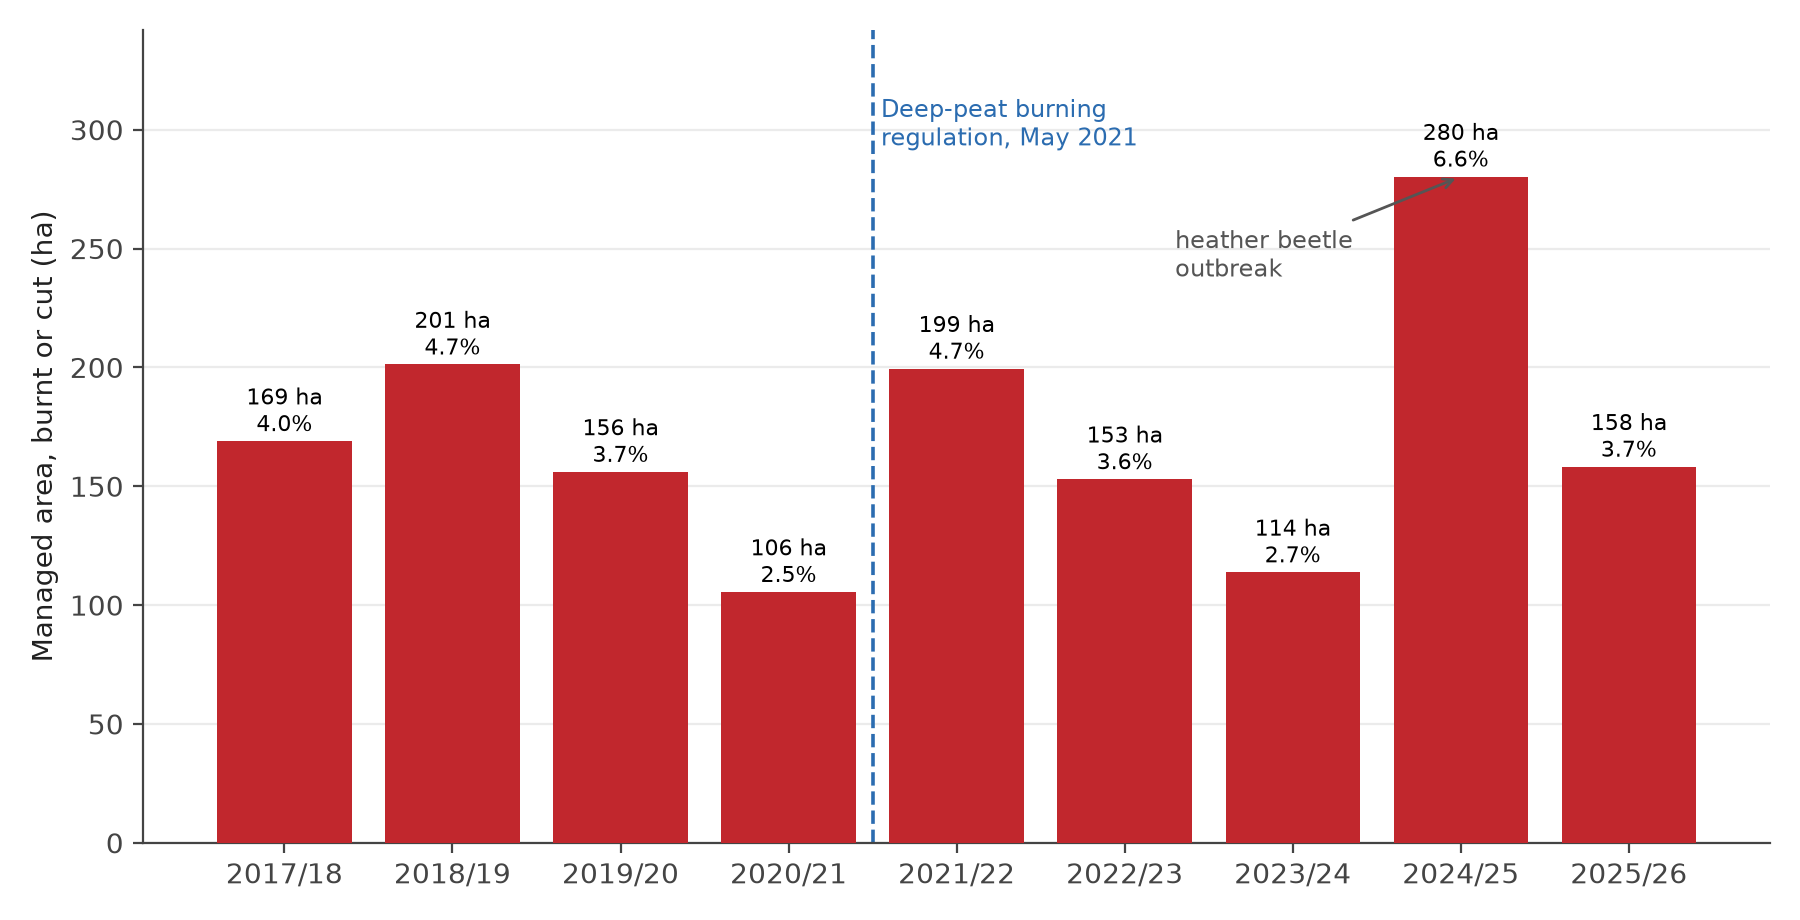
\includegraphics[width=0.92\linewidth]{fig_season_totals.png}
\caption{Ground burnt or cut within the 28 count areas, by season. The dashed line marks the deep-peat burning regulation of May 2021.}\label{fig:seasons}
\end{figure}

\begin{table}[htbp]
\centering
\caption{Ground burnt or cut by season.}\label{tab:seasons}
\small
\begin{threeparttable}
\begin{tabular}{lrrr}
\toprule
Season & Burnt or cut (ha) & \% of count area & Clear images per pixel\textsuperscript{a} \\
\midrule
2017/18 & 169 & 4.0 & 11.2 \\
2018/19 & 201 & 4.7 & 5.5 \\
2019/20 & 156 & 3.7 & 8.2 \\
2020/21 & 106 & 2.5 & 8.6 \\
2021/22 & 199 & 4.7 & 4.9 \\
2022/23 & 153 & 3.6 & 6.7 \\
2023/24 & 114 & 2.7 & 4.8 \\
2024/25 & 280 & 6.6 & 9.1 \\
2025/26 & 158 & 3.7 & 7.7 \\
\midrule
\textbf{Mean} & \textbf{171} & \textbf{4.0} & 7.5 \\
\bottomrule
\end{tabular}

\begin{tablenotes}\footnotesize
\item[a] Median over count areas of the clear after-season scenes per pixel; the mean row gives the median over all count-area seasons.
\end{tablenotes}
\end{threeparttable}
\end{table}

On average \textbf{171~ha, 4.0\% of the count area, was burnt or cut each season} (\figref{fig:seasons}, \tabref{tab:seasons}). Seasons range from 106~ha (2.5\%) in 2020/21 to 280~ha (6.6\%) in 2024/25.

\subsection{Count areas and moors}\label{sec:areas}

\begin{figure}[htbp]
\centering
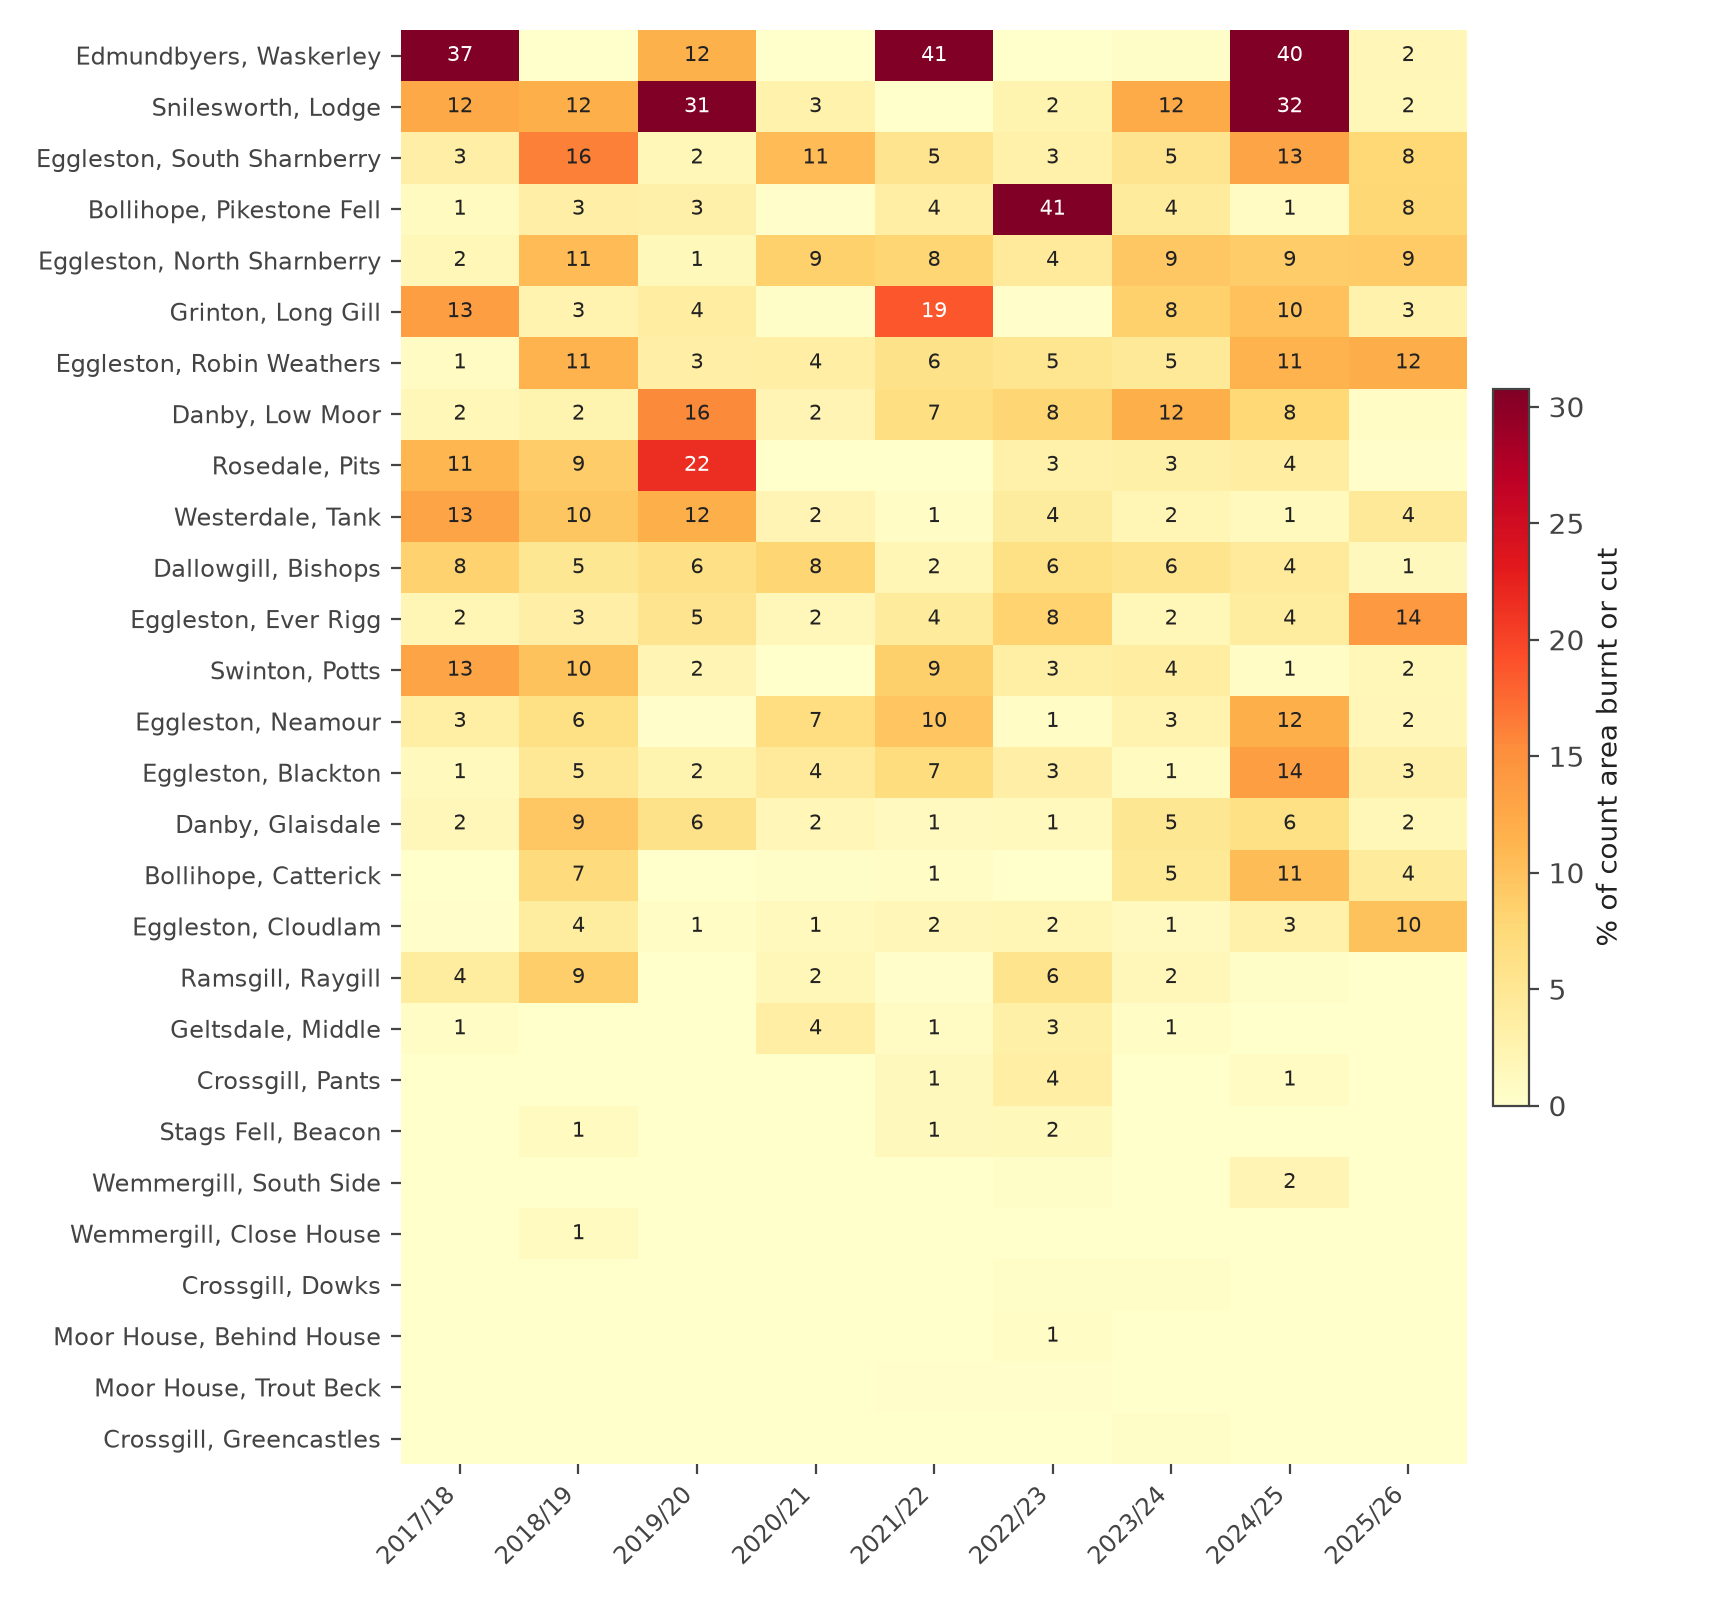
\includegraphics[width=0.86\linewidth]{fig_heatmap.png}
\caption{Percentage of each count area burnt or cut, by season. Values of 0.5\% or more are printed. Count areas are ordered by their mean.}\label{fig:heatmap}
\end{figure}

\figref{fig:heatmap} shows the \textbf{sporadic pattern} PW described. Edmundbyers, Waskerley was heavily managed in four seasons (37\%, 12\%, 41\% and 40\%) and barely touched in the other five. Snilesworth, Lodge shows the same pattern. Most other working moors manage a few per cent of each count area in most seasons.

The imagery shows what a heavy season looks like (\figref{fig:waskerley}). At Waskerley the managed ground in each heavy season is many small patches spread across the count area: the mosaic of rotational burning and cutting, not a single event.

\begin{figure}[htbp]
\centering
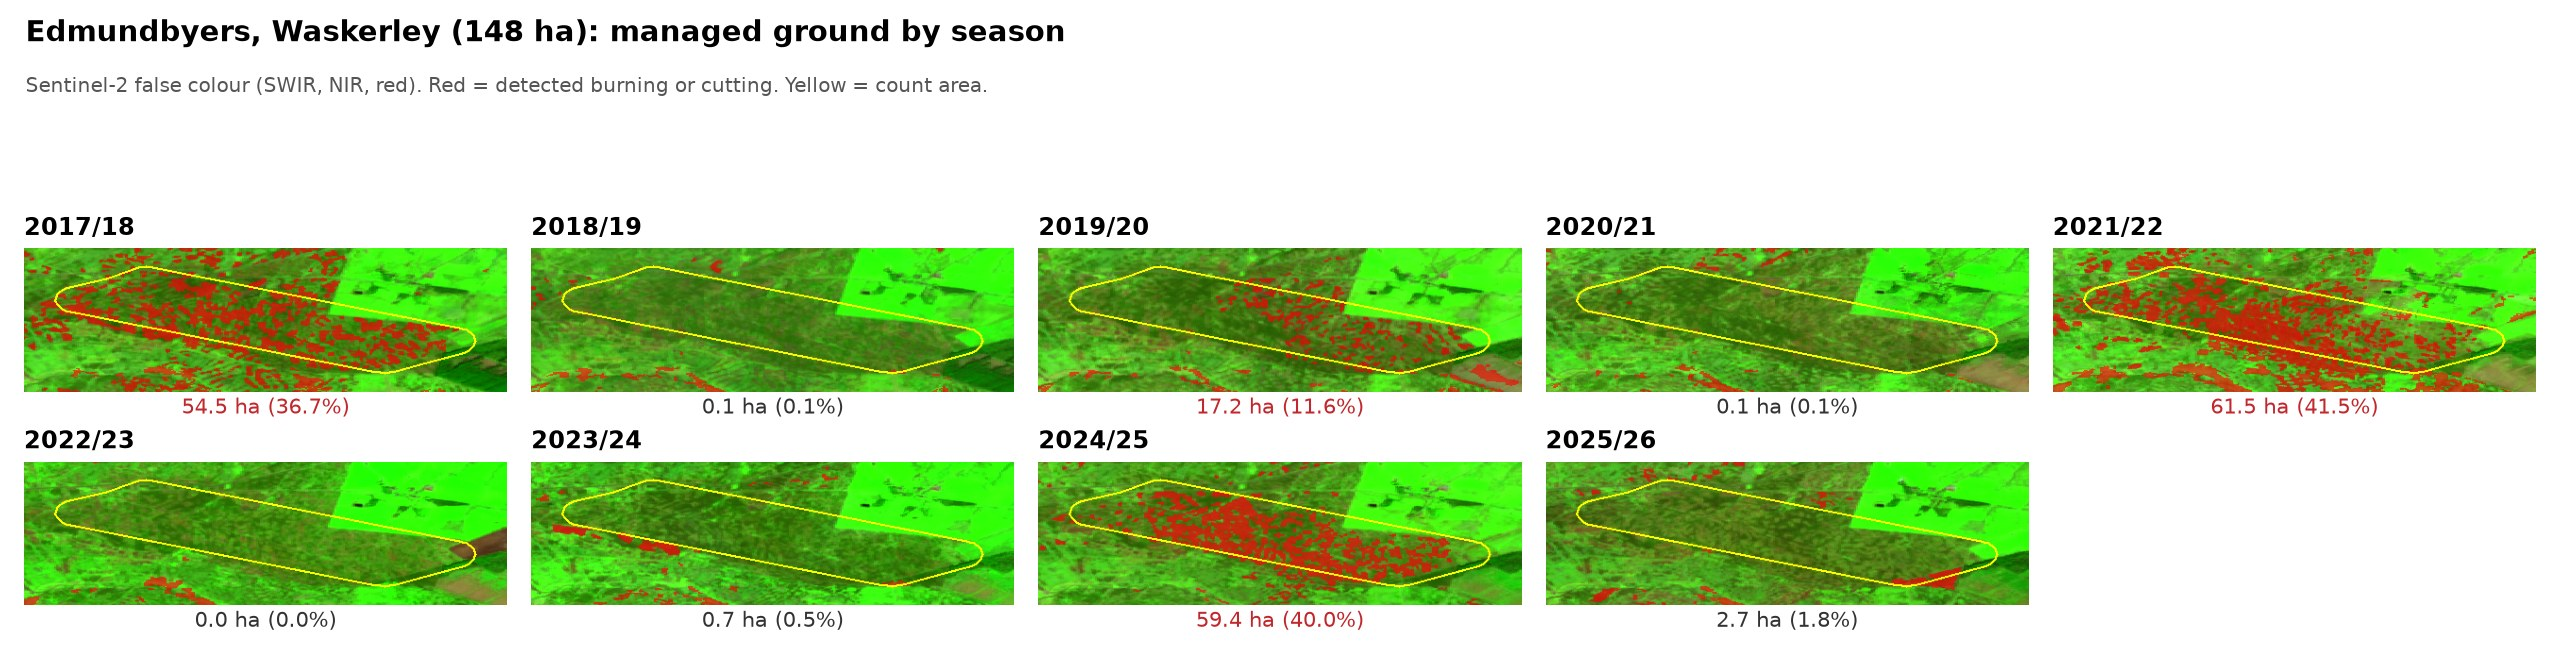
\includegraphics[width=\linewidth]{Edmundbyers_Waskerley.jpg}
\caption{Edmundbyers, Waskerley, season by season. Sentinel-2 false colour after each season; red is ground detected as burnt or cut; yellow is the count area.}\label{fig:waskerley}
\end{figure}

One single event stands out: \textbf{Bollihope, Pikestone Fell, 41\% in 2022/23}, against 0 to 8\% in every other season (version~1 also found it). Unlike Waskerley's mosaic, it is one solid block of about 40~ha, far larger than a normal rotational burn of 2 to 5~ha (\figref{fig:pikestone}). It may have been a wildfire and is worth checking with the estate.

\begin{figure}[htbp]
\centering
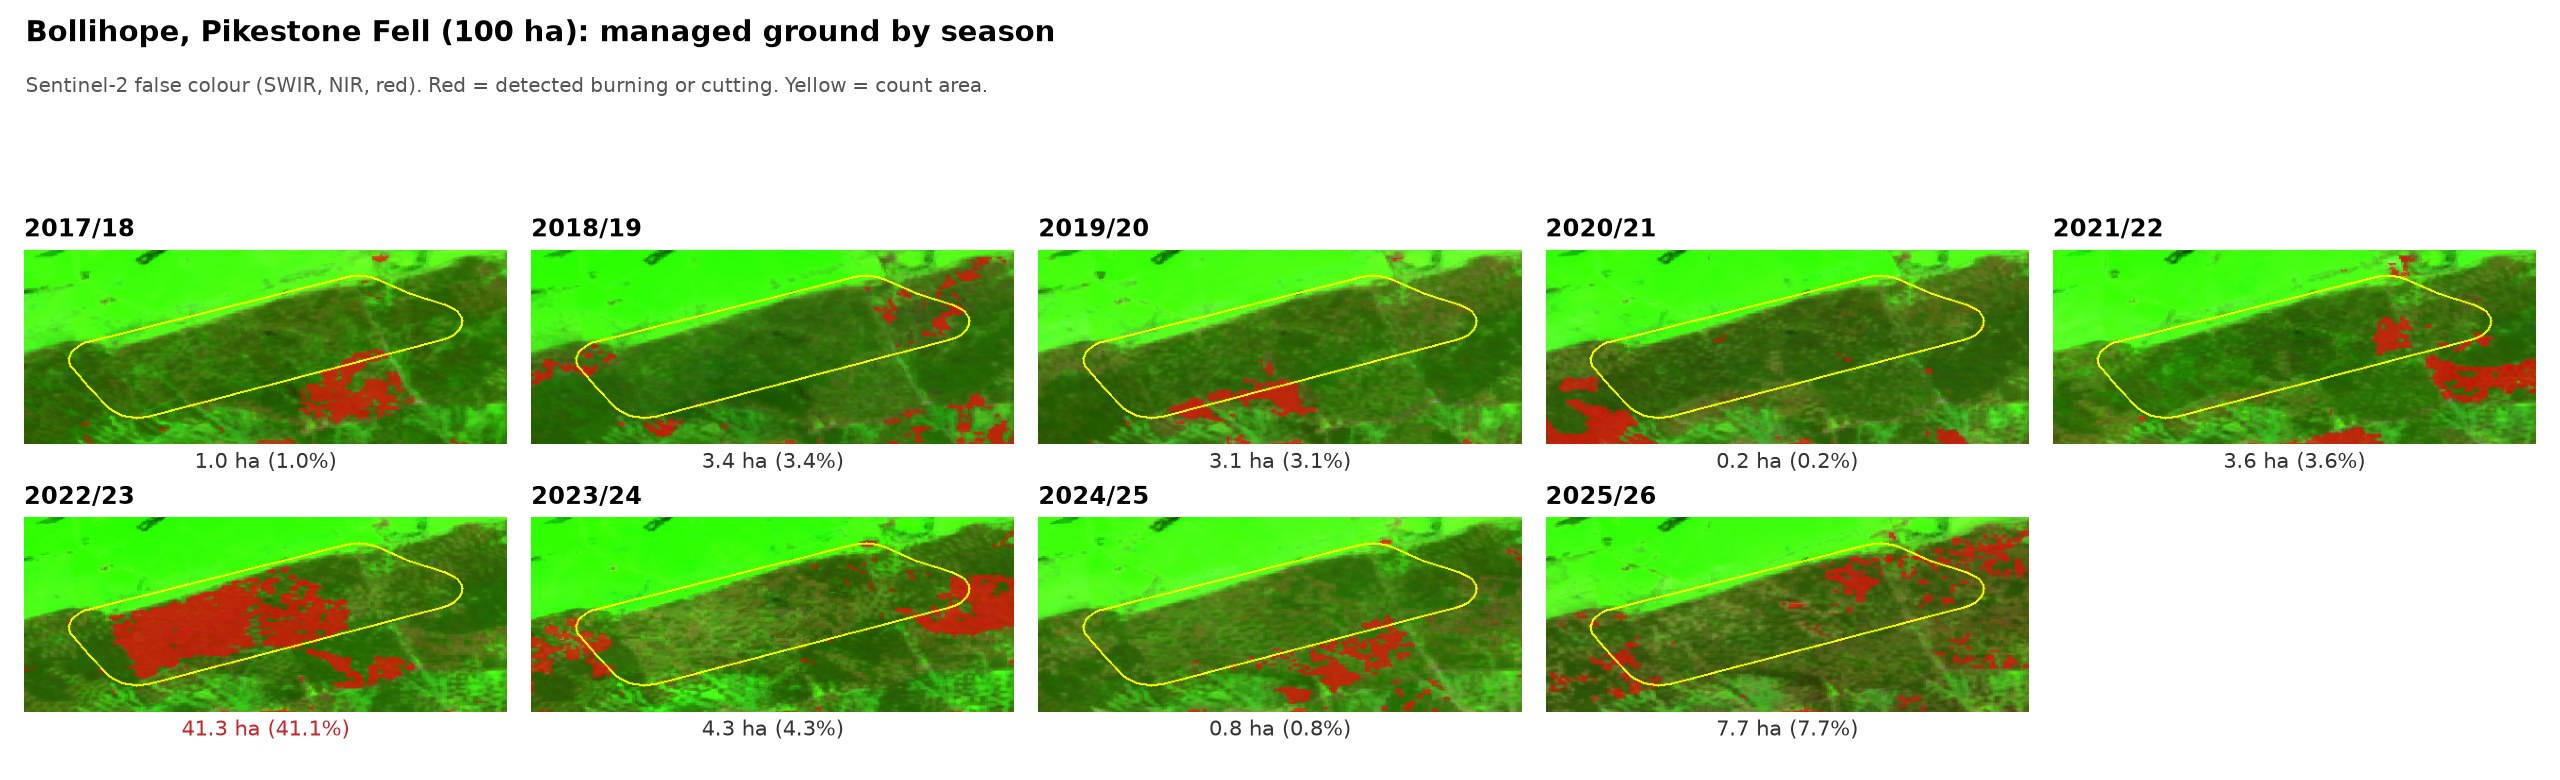
\includegraphics[width=\linewidth]{Bollihope_PikestoneFell.jpg}
\caption{Bollihope, Pikestone Fell, season by season. The 2022/23 detection is a single block of about 40~ha.}\label{fig:pikestone}
\end{figure}

\needspace{12\baselineskip}
By moor (\figref{fig:map}, \tabref{tab:moors}), Edmundbyers (14.7\% a year) and Snilesworth (11.8\%) are the most intensively managed. Five moors are at or below 1\%: Geltsdale, Stags Fell, Crossgill, Wemmergill and Moor House. Grinton's 6.7\% rests partly on two seasons with very few clear images (2021/22 and 2024/25).

\begin{figure}[htbp]
\centering
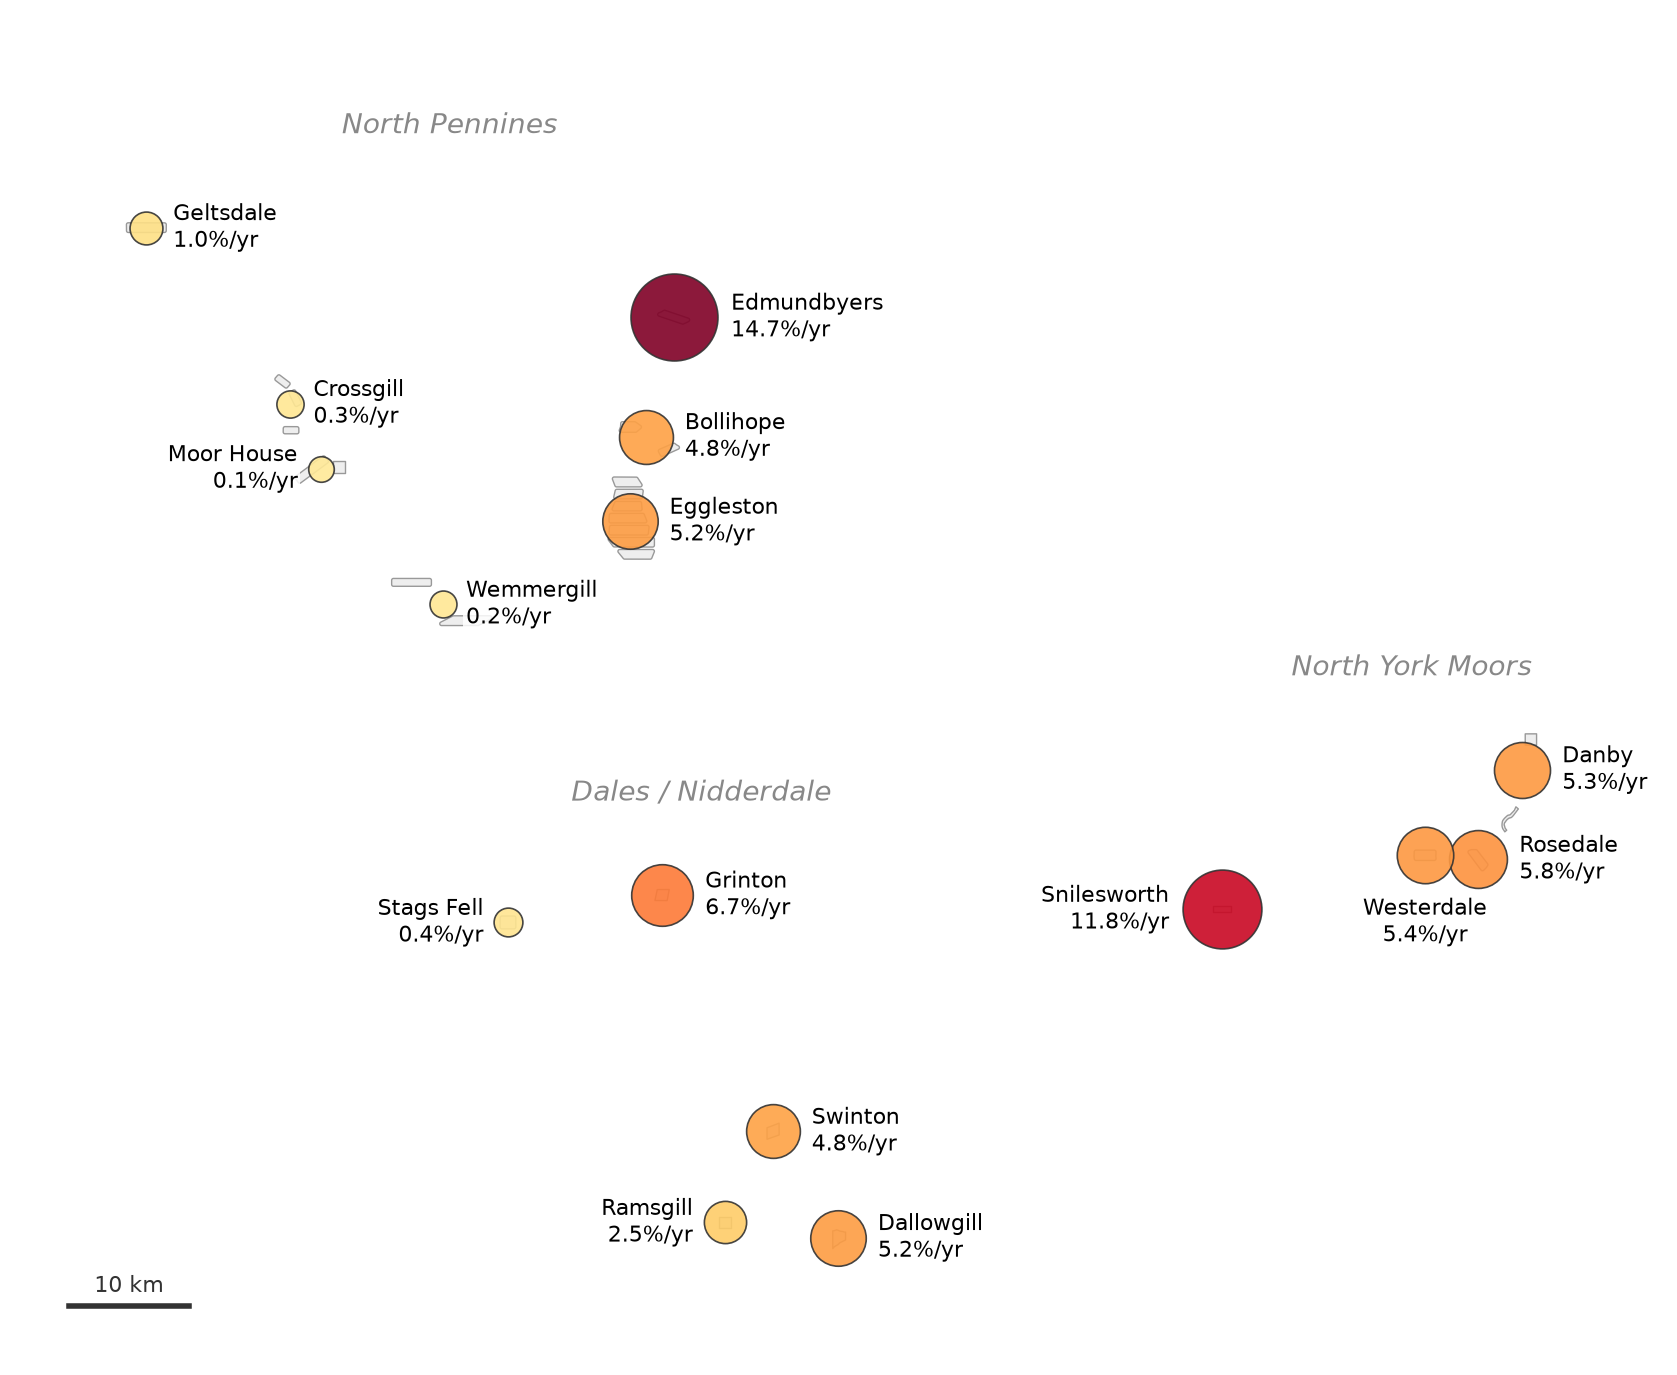
\includegraphics[width=0.74\linewidth]{fig_map.png}
\caption{Mean annual percentage of count area burnt or cut, by moor. Circle size and colour show the percentage.}\label{fig:map}
\end{figure}

\begin{table}[htbp]
\centering
\caption{Mean annual percentage of count area burnt or cut, by moor.}\label{tab:moors}
\small
\begin{tabular}{llrrr}
\toprule
Moor & Region & Count areas & Area (ha) & Mean \% a year \\
\midrule
Edmundbyers & North Pennines & 1 & 148 & 14.7 \\
Snilesworth & North York Moors & 1 & 73 & 11.8 \\
Grinton & Dales and Nidderdale & 1 & 91 & 6.7 \\
Rosedale & North York Moors & 1 & 139 & 5.8 \\
Westerdale & North York Moors & 1 & 153 & 5.4 \\
Danby & North York Moors & 2 & 142 & 5.3 \\
Dallowgill & Dales and Nidderdale & 1 & 112 & 5.2 \\
Eggleston & North Pennines & 7 & 1,557 & 5.2 \\
Bollihope & North Pennines & 2 & 237 & 4.8 \\
Swinton & Dales and Nidderdale & 1 & 97 & 4.8 \\
Ramsgill & Dales and Nidderdale & 1 & 92 & 2.5 \\
Geltsdale & North Pennines & 1 & 263 & 0.98 \\
Stags Fell & Dales and Nidderdale & 1 & 137 & 0.45 \\
Crossgill & North Pennines & 3 & 225 & 0.26 \\
Wemmergill & North Pennines & 2 & 496 & 0.23 \\
Moor House & North Pennines & 2 & 310 & 0.08 \\
\bottomrule
\end{tabular}

\end{table}

\subsection{Regional pattern}\label{sec:regions}

\begin{table}[htbp]
\centering
\caption{Mean annual percentage burnt or cut by region, against \citet{shewring2024}.}\label{tab:regions}
\small
\begin{tabular}{lll}
\toprule
Region & This study (burnt or cut) & \citet{shewring2024} (burnt only) \\
\midrule
North York Moors & 6.4\% a year & about 6.3\% a year \\
North Pennines & 3.7\% a year & about 2.7\% a year \\
Yorkshire Dales and Nidderdale & 3.7\% a year & not compared \\
\bottomrule
\end{tabular}
\end{table}

The ordering matches \citet{shewring2024}, and the North York Moors figure is almost identical (\tabref{tab:regions}). The North Pennines figure is higher than theirs. Our figure includes cutting and theirs does not, and with cutting replacing burning on blanket bog since 2021 a higher figure is expected. The two studies also cover different areas: count areas here, whole regions there.

\subsection{Before and after the 2021 regulation}\label{sec:regulation}

\begin{table}[htbp]
\centering
\caption{Mean ground burnt or cut per season, by period.}\label{tab:regulation}
\small
\begin{tabular}{lr}
\toprule
Period & Burnt or cut per season \\
\midrule
2017/18 to 2020/21 (before) & 158~ha (3.7\%) \\
2021/22 to 2023/24 (after) & 155~ha (3.6\%) \\
2024/25 (beetle outbreak) & 280~ha (6.6\%) \\
2025/26 & 158~ha (3.7\%) \\
\bottomrule
\end{tabular}
\end{table}

Total management held steady after the regulation (\tabref{tab:regulation}). This is consistent with PW's field observation that estates on blanket bog switched from burning to cutting, which is not limited by weather. It is also compatible with the 73\% fall in burning in \citet{shewring2024}, which does not count cutting. The satellite measures burning and cutting together, so it shows the total holding steady; the field observations show the switch within it.

\subsection{The 2024/25 peak}\label{sec:2024}

\textbf{2024/25 is the highest season in the record.} Without Sentinel-2C scenes it is 252~ha, 10\% lower but still well above the next highest season (201~ha), and the ranking of count areas barely changes (rank correlation 0.97). It is the highest season at every threshold, and under every combination of boundaries, window and patch size tested in \secref{sec:review}.

The peak coincides with the heather beetle outbreak and fits PW's observation that managers burnt and cut beetle-killed heather to promote recovery. Count areas with more damage in the July 2025 survey were more heavily managed in 2024/25 (rank correlation 0.55). They were also the more heavily managed ones before the outbreak (0.70 in 2023/24), and relative to each count area's usual level the 2024/25 increase is spread across count areas. Damage records from 2024, the summer before managers responded, would allow the response to be traced count area by count area.

Beetle-related management may also be under-counted. Burning or cutting heather that is already dead changes the satellite signal less than burning live heather. This may be why the count areas with the heaviest damage show less management than usual in 2025/26 (rank correlation $-0.40$ relative to their usual level).

\subsection{Robustness}\label{sec:robust}

\begin{figure}[htbp]
\centering
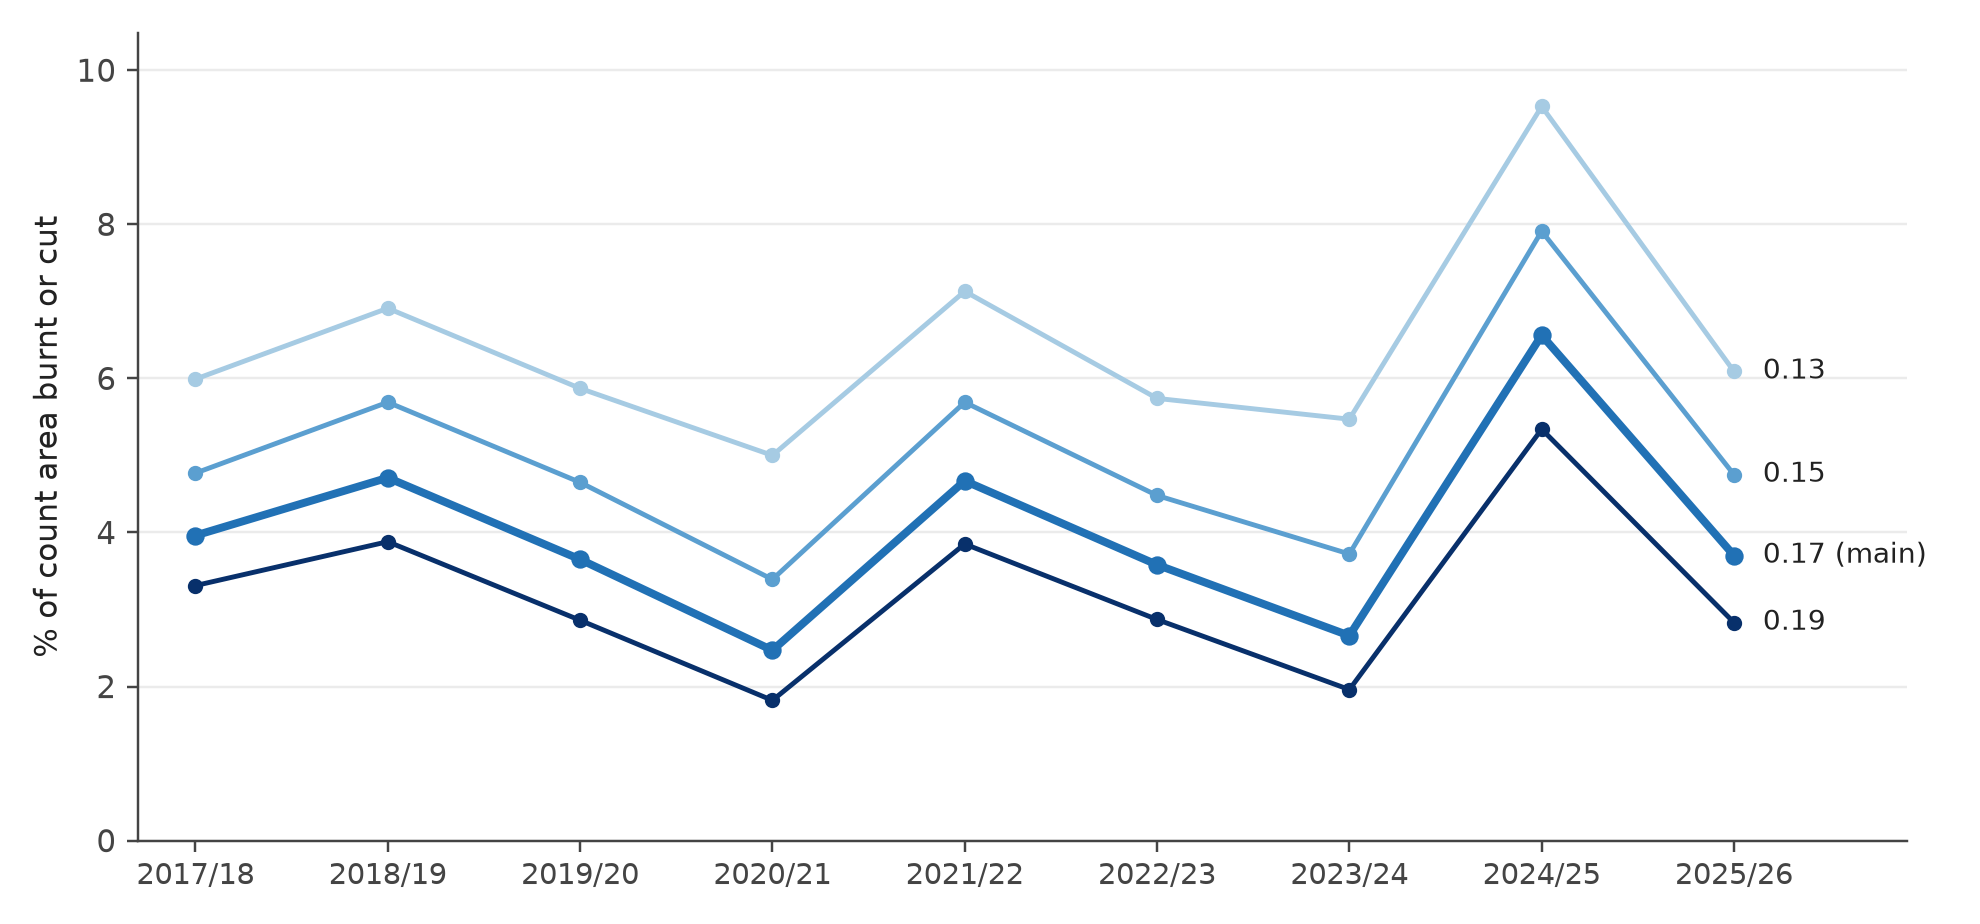
\includegraphics[width=0.88\linewidth]{fig_threshold_sensitivity.png}
\caption{Percentage of count area burnt or cut by season at four thresholds. Levels shift; the pattern does not.}\label{fig:thresholds}
\end{figure}

Between thresholds of 0.15 and 0.19 the totals change by about a fifth, but every pattern in this report holds (\figref{fig:thresholds}). The order of seasons and moors agrees with the main run (rank correlations 0.93 to 1.00). The North York Moors stay 1.6 to 1.8 times the North Pennines, and the after/before 2021 ratio stays between 0.97 and 1.03. At 0.13 the reserves start to register (Geltsdale 4.5\% a year), so 0.13 is too permissive. The full table is in \appref{app:thresholds}.

\begin{table}[htbp]
\centering
\caption{Checks on the results.}\label{tab:checks}
\small
\begin{tabularx}{\linewidth}{>{\raggedright\arraybackslash}p{0.27\linewidth}>{\raggedright\arraybackslash}p{0.22\linewidth}L}
\toprule
Check & Expected & Result \\
\midrule
Moor House (National Nature Reserve) & Near zero & 0.08\% a year \\
Geltsdale (RSPB reserve) & Low & 1.0\% a year \\
North York Moors against North Pennines & NYM higher \citep{shewring2024} & 6.4\% against 3.7\% \\
Crossgill and Wemmergill & More than Geltsdale (PW) & 0.26\% and 0.23\%: their cuts are mostly smaller than 0.1~ha, as PW anticipated \\
2024/25 and Sentinel-2C & Similar without it & 252 against 280~ha, still the highest \\
Eggleston as one block & Similar & 5.3\% against 5.2\% \\
\bottomrule
\end{tabularx}
\end{table}

% ================================================================ 5 review
\section{What the review changed}\label{sec:review}

\subsection{Effect of each change}\label{sec:ablation}

\figref{fig:ablation} and \tabref{tab:ablation} show the analysis re-run one change at a time on the 27 count areas the two versions share.

\begin{figure}[htbp]
\centering
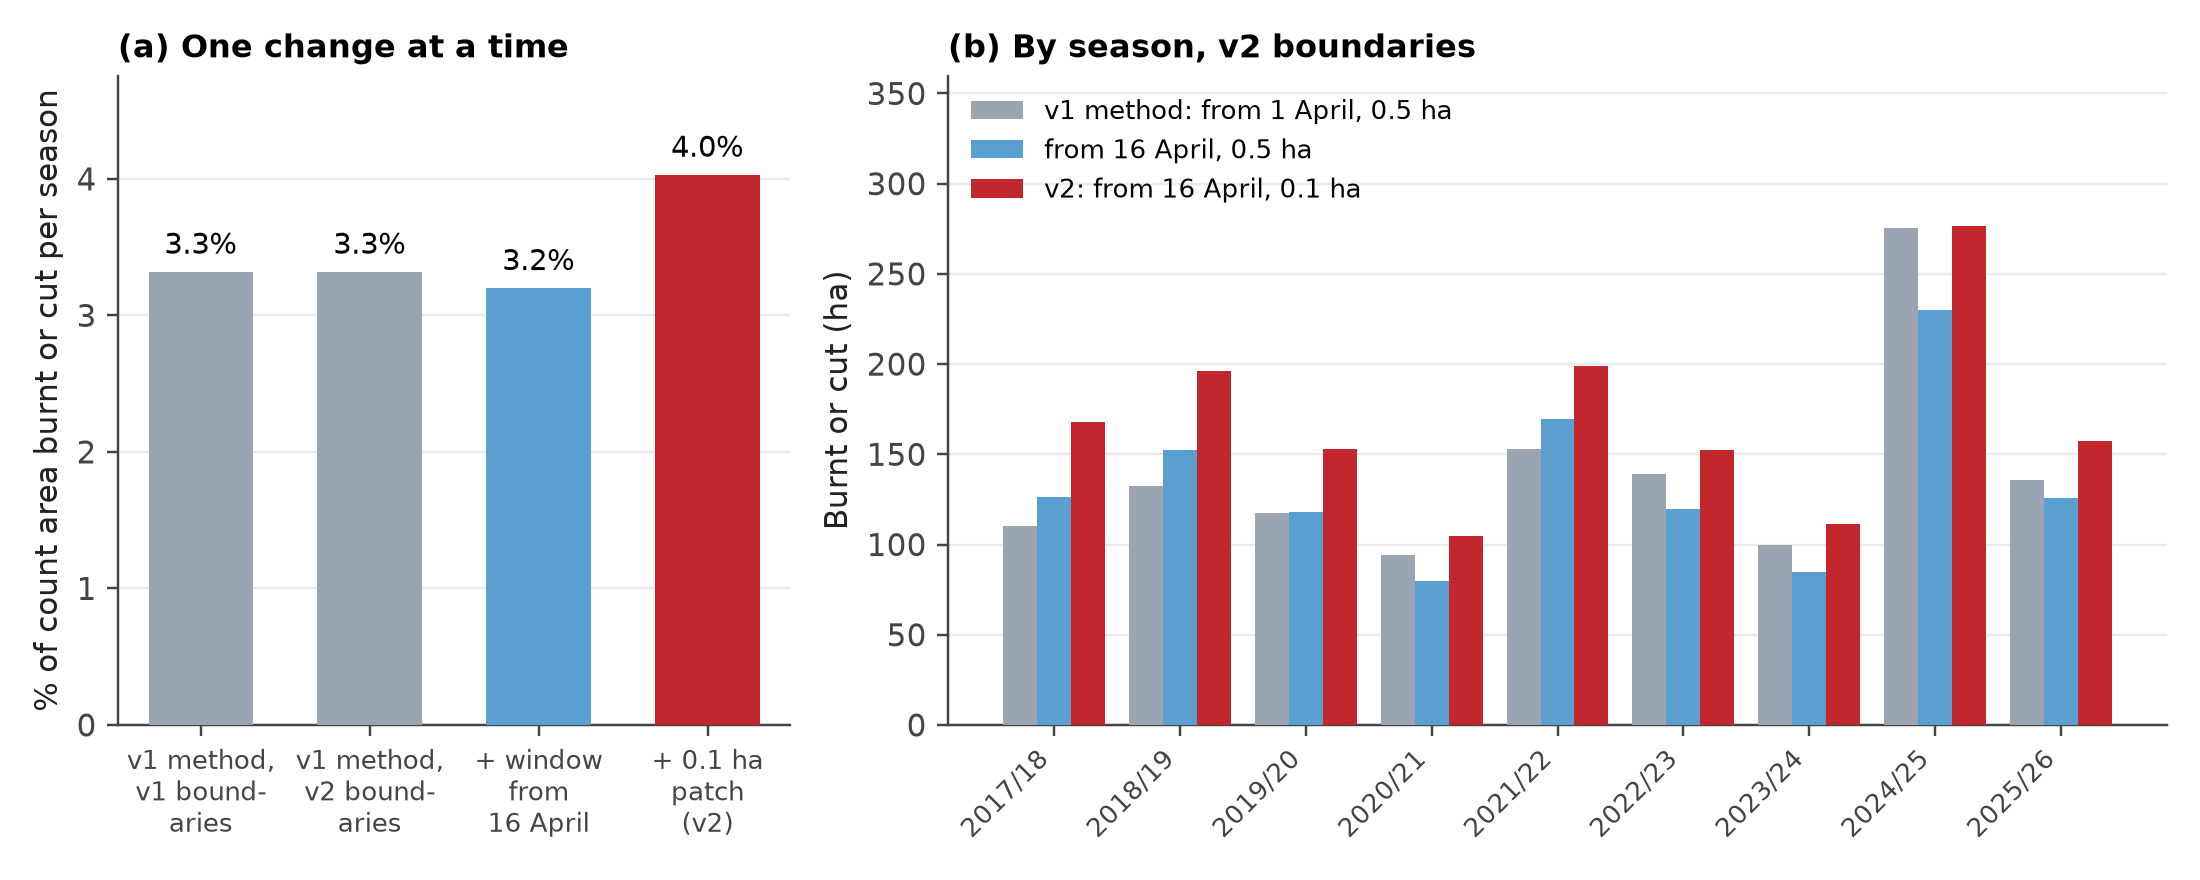
\includegraphics[width=\linewidth]{fig_v5_to_v6.png}
\caption{(a) Mean percentage burnt or cut per season on the 27 shared count areas, 2017/18 to 2024/25, as each change is added. (b) Hectares by season on the same count areas with version~2 boundaries: the version~1 method, the new window alone (16 April to 30 June), and version~2.}\label{fig:ablation}
\end{figure}

\begin{table}[htbp]
\centering
\caption{The analysis with one change at a time: 27 count areas, 2017/18 to 2024/25.}\label{tab:ablation}
\footnotesize
\setlength{\tabcolsep}{4pt}
\begin{threeparttable}
\begin{tabular}{llrrrrr}
\toprule
Run & After window & \makecell[r]{Min.\\patch (ha)} & \makecell[r]{\%\\a year} & \makecell[r]{Seasons with\\none (\%)} & \makecell[r]{Seven\\areas (ha)\textsuperscript{a}} & \makecell[r]{2024/25\\(ha)} \\
\midrule
\multicolumn{7}{l}{\textit{Version 1 boundaries (2,546 ha)}} \\
Version 1 as published (main class) & 1 Apr to 31 May & 0.5 & 3.3 & 41 & 211 & 175 \\
Version 1 method, rebuilt here & 1 Apr to 31 May & 0.5 & 3.3 & 41 & 213 & 175 \\
Version 2 method & 16 Apr to 30 Jun & 0.1 & 4.2 & 29 & 284 & 178 \\
\midrule
\multicolumn{7}{l}{\textit{Version 2 boundaries (4,218 ha)}} \\
Version 1 method & 1 Apr to 31 May & 0.5 & 3.3 & 35 & 219 & 275 \\
\quad start on 16 April only & 16 Apr to 31 May & 0.5 & 3.2 & 33 & 230 & 252 \\
\quad start on 16 April, end on 30 June & 16 Apr to 30 Jun & 0.5 & 3.2 & 34 & 215 & 230 \\
\quad 0.1 ha patch only & 1 Apr to 31 May & 0.1 & 4.2 & 25 & 302 & 319 \\
\textbf{Version 2} & 16 Apr to 30 Jun & 0.1 & 4.0 & 23 & 291 & 277 \\
\bottomrule
\end{tabular}

\begin{tablenotes}\footnotesize
\item[a] Total over the eight seasons on Dallowgill, Ramsgill, Swinton, Grinton, Snilesworth, Danby Low Moor and Moor House Behind House, whose boundaries barely changed.
\end{tablenotes}
\end{threeparttable}
\end{table}

\begin{itemize}
\item \textbf{The rebuild reproduces version~1:} 3.3\% a year, 41\% of count-area seasons with nothing detected, and 213~ha against 211~ha on the seven unchanged count areas. The comparison starts from a faithful copy.
\item \textbf{The boundaries change the hectares, not the percentages.} On Eleanor's boundaries the count areas cover 4,218~ha instead of 2,546~ha, but the share managed stays at 3.3\%. Fewer seasons show nothing (35\%), because larger areas are less likely to be untouched.
\item \textbf{Starting the after window on 16 April changes little on its own:} 3.3\% to 3.2\% a year. On the seven unchanged count areas it adds 5\% (219 to 230~ha), consistent with some early-April work now being counted in full. Most early-April work was already counted, because the after image is the median of many scenes, most of them taken after the work.
\item \textbf{Ending the window on 30 June rather than 31 May moves ground between seasons} without changing the total (3.2\%; \figref{fig:ablation}b). The extra June scenes change which scars stand out in some seasons.
\item \textbf{The 0.1~ha minimum patch has the largest effect.} On its own it raises the figure from 3.3\% to 4.2\% a year and cuts the seasons with nothing detected from 35\% to 25\%. Many fires and cuts are small, as PW said.
\item \textbf{With all the changes} the figure is 4.0\% a year, and 23\% of count-area seasons show nothing.
\end{itemize}

\subsection{Version~1's late detections}\label{sec:late}

Version~1 also reported a second, ``late'' class: ground that changed only between the after window and late summer. PW suggested these were the season's early-April burns. On the seven unchanged count areas, version~1 found 211~ha in its main class and 65~ha in the late class, close to version~2's 291~ha. The runs above show that starting the window on 16 April adds little on its own, so the late class was not mainly early-April work.

The timing points elsewhere. Over half of the late class (91 of 165~ha) falls in 2023/24 and 2024/25, whose late-summer images are from summers 2024 and 2025, during the beetle outbreak. In those two seasons 88 of its 91~ha lie on count areas the July 2025 survey scored 0.3 or more, and it follows the survey's damage (rank correlation 0.51 and 0.50, against $-0.06$ in 2022/23). \textbf{Most of version~1's late detections were probably heather beetle browning.} Version~2 does not count them as management; the beetle damage is now measured separately (\secref{sec:beetle}).

\subsection{Review points and responses}

\begin{table}[htbp]
\centering
\caption{PW's review of version~1, what version~2 does, and what it showed.}\label{tab:review}
\footnotesize
\begin{tabularx}{\linewidth}{>{\raggedright\arraybackslash}p{0.29\linewidth}>{\raggedright\arraybackslash}p{0.25\linewidth}L}
\toprule
PW's review & Version 2 & What it showed \\
\midrule
The season ends on 15 April; early April is often the busiest & After window from 16 April & Early-April work is fully counted; totals move little (\secref{sec:ablation}) \\
Many fires and cuts are small, sometimes 10~m by 20~m & Minimum patch 0.1~ha & The largest single effect: 3.3\% to 4.2\% a year \\
Burning and cutting both happen October to 15 April & One class, burnt or cut & Timing cannot separate them; aerial imagery can \\
Every season is usable; management is sporadic & Every season reported & The heavy-then-light pattern is confirmed in the imagery (\figref{fig:waskerley}) \\
After 2021, blanket bog estates cut instead of burning & Total management reported & Total holds steady after 2021 (\secref{sec:regulation}) \\
2024/25 reflects management of beetle-killed heather & Included and tested & Highest season under every test (\secref{sec:2024}) \\
More cutting expected at Crossgill and Wemmergill & 0.1~ha patch; image sheets & Still 0.2 to 0.3\%: the cuts are mostly below 0.1~ha \\
The late (blue) scars are early-April burns & Window from 16 April & Late detections were mostly beetle browning (\secref{sec:late}) \\
Definitive boundaries available & Eleanor's polygons & Percentages unchanged; hectares larger \\
Map did not show the proportion & Circles sized by percentage, plus a table & \figref{fig:map} and \figref{fig:heatmap} \\
\bottomrule
\end{tabularx}
\end{table}

% ================================================================ 6 beetle
\section{Heather beetle damage}\label{sec:beetle}

\subsection{Agreement with the survey}

\begin{figure}[htbp]
\centering
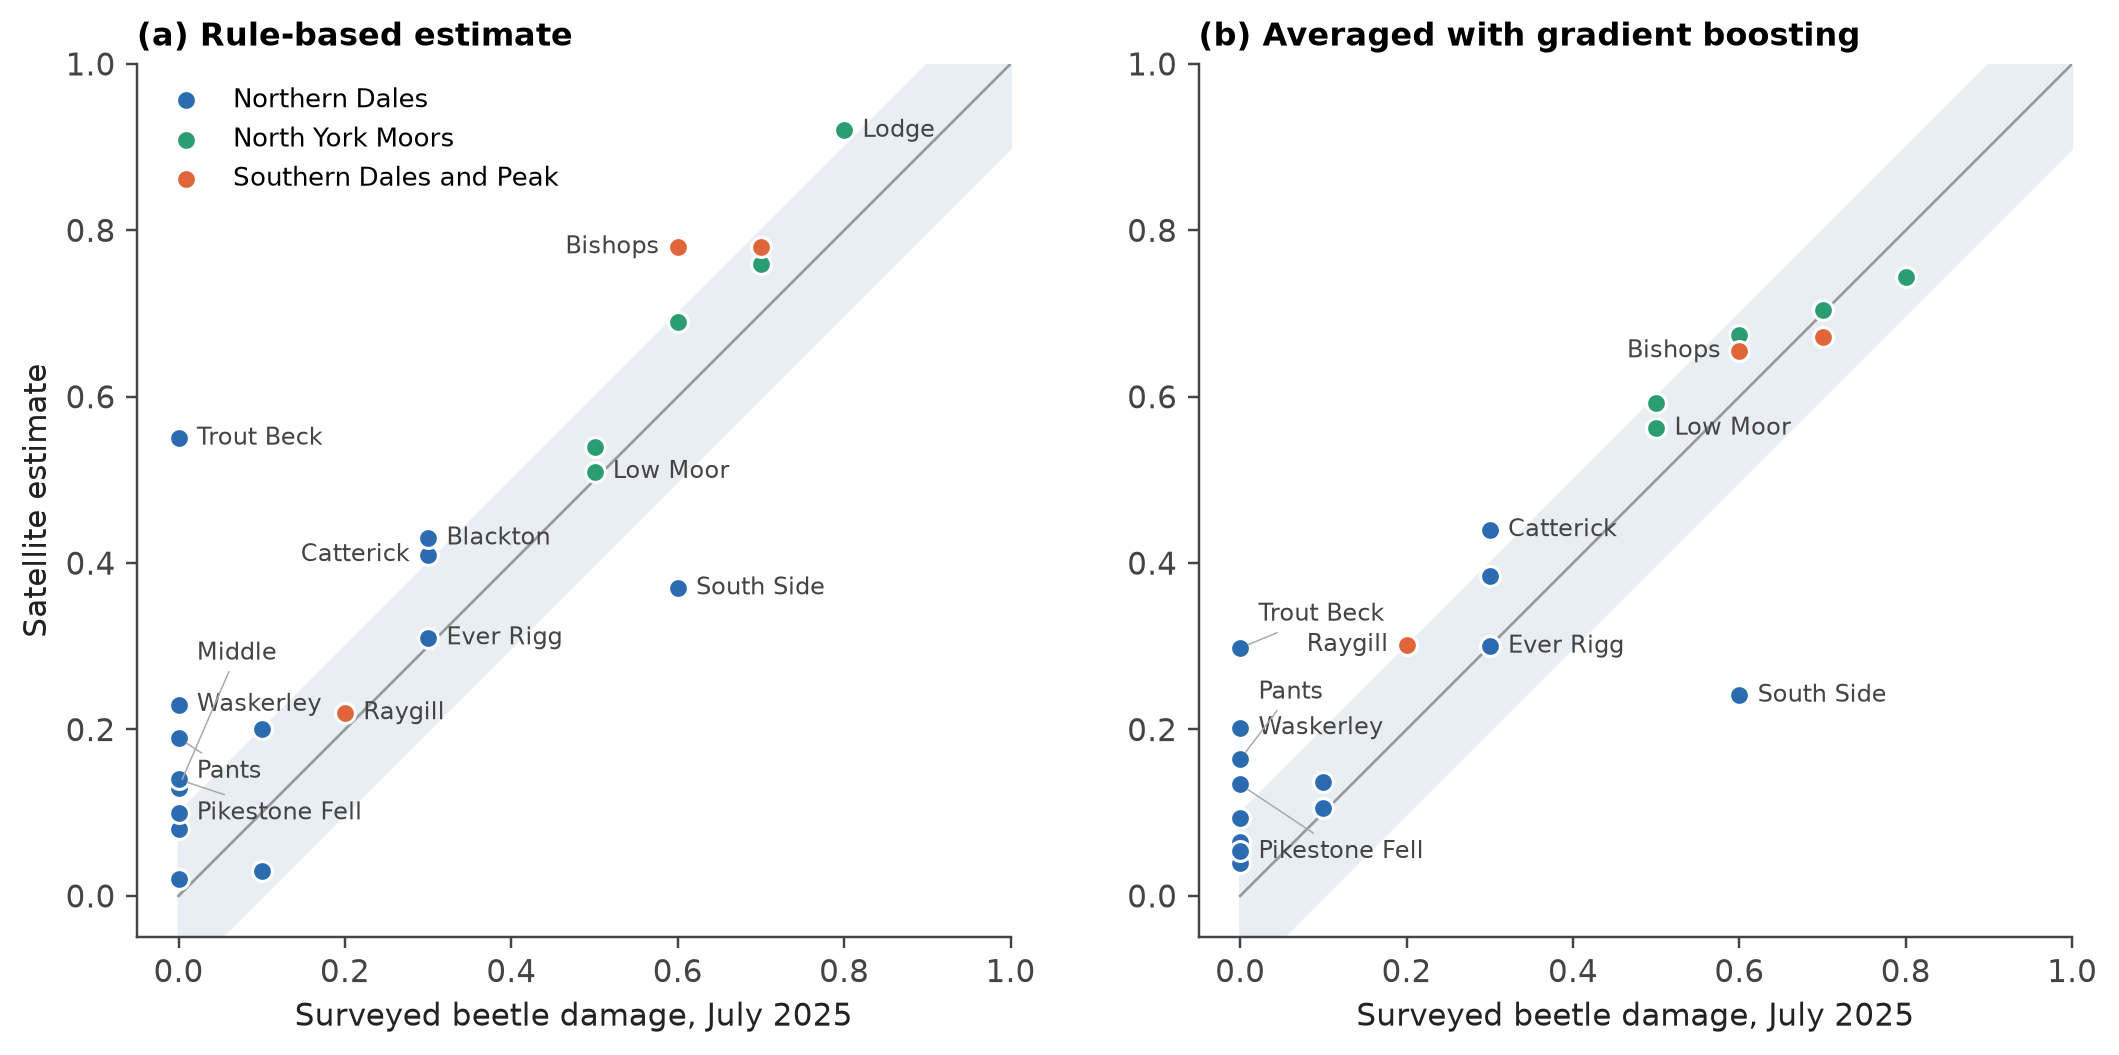
\includegraphics[width=\linewidth]{fig_beetle_gb.png}
\caption{Satellite estimates of heather beetle damage against the July 2025 survey: (a) the rule-based estimate; (b) the rule-based estimate averaged with gradient boosting. Each moor is predicted without its own data. The shaded band is within 0.1 of the survey. Count areas more than 0.1 from the survey, or discussed in the text, are labelled.}\label{fig:beetle}
\end{figure}

\begin{table}[htbp]
\centering
\caption{Agreement between the satellite estimate and the survey, 22 count areas, each moor predicted without its own data.}\label{tab:beetle}
\small
\begin{threeparttable}
\begin{tabular}{lccc}
\toprule
 & \makecell{Region\\average\tnote{a}} & \makecell{Rule-based\\estimate} & \makecell{\textbf{Rule +}\\\textbf{gradient boosting}} \\
\midrule
Typical difference from the survey & 0.17 & 0.12 & \textbf{0.10} \\
Within 0.1 of the survey & & 12 of 22 & \textbf{15 of 22} \\
Within 0.2 of the survey & & 19 of 22 & \textbf{19 of 22} \\
Rank agreement (Spearman's $\rho$) & & 0.81 & \textbf{0.88} \\
\bottomrule
\end{tabular}
\begin{tablenotes}\footnotesize
\item[a] Each count area predicted as the average damage of the other moors in its region, with no satellite data.
\end{tablenotes}
\end{threeparttable}
\end{table}

The combined estimate is \textbf{within 0.1 of the survey on 15 of 22 count areas and within 0.2 on 19}, with a typical difference of 0.10 (\figref{fig:beetle}, \tabref{tab:beetle}). It ranks the count areas almost as the survey does (0.88). Values for every count area are in \appref{app:beetle-areas}.

\subsection{What the satellite sees}

\begin{itemize}
\item \textbf{The rule captures the full range of damage.} Close matches include Danby, Low Moor (0.51 against 0.5), Eggleston, Ever Rigg (0.31 against 0.3) and Ramsgill, Raygill (0.22 against 0.2). Greying matters: Dallowgill, Bishops (survey 0.6) barely browned but greyed strongly.
\item \textbf{Gradient boosting learns what is not damage.} At Moor House, Trout Beck the rule reads 0.55 against a survey score of 0, because the whole bog changed colour. Gradient boosting learned from the undamaged count areas that this greying is not damage and reads 0.05; the average is 0.30.
\item \textbf{The red-edge bands carry much of the signal.} After the change in NBR between early and late summer 2025, the measures gradient boosting relies on most are the red-edge bands B5 and B6, which respond to the loss of chlorophyll. Four of its ten most-used measures are red-edge (\figref{fig:importance}).
\item[] \begin{minipage}{\linewidth}\centering
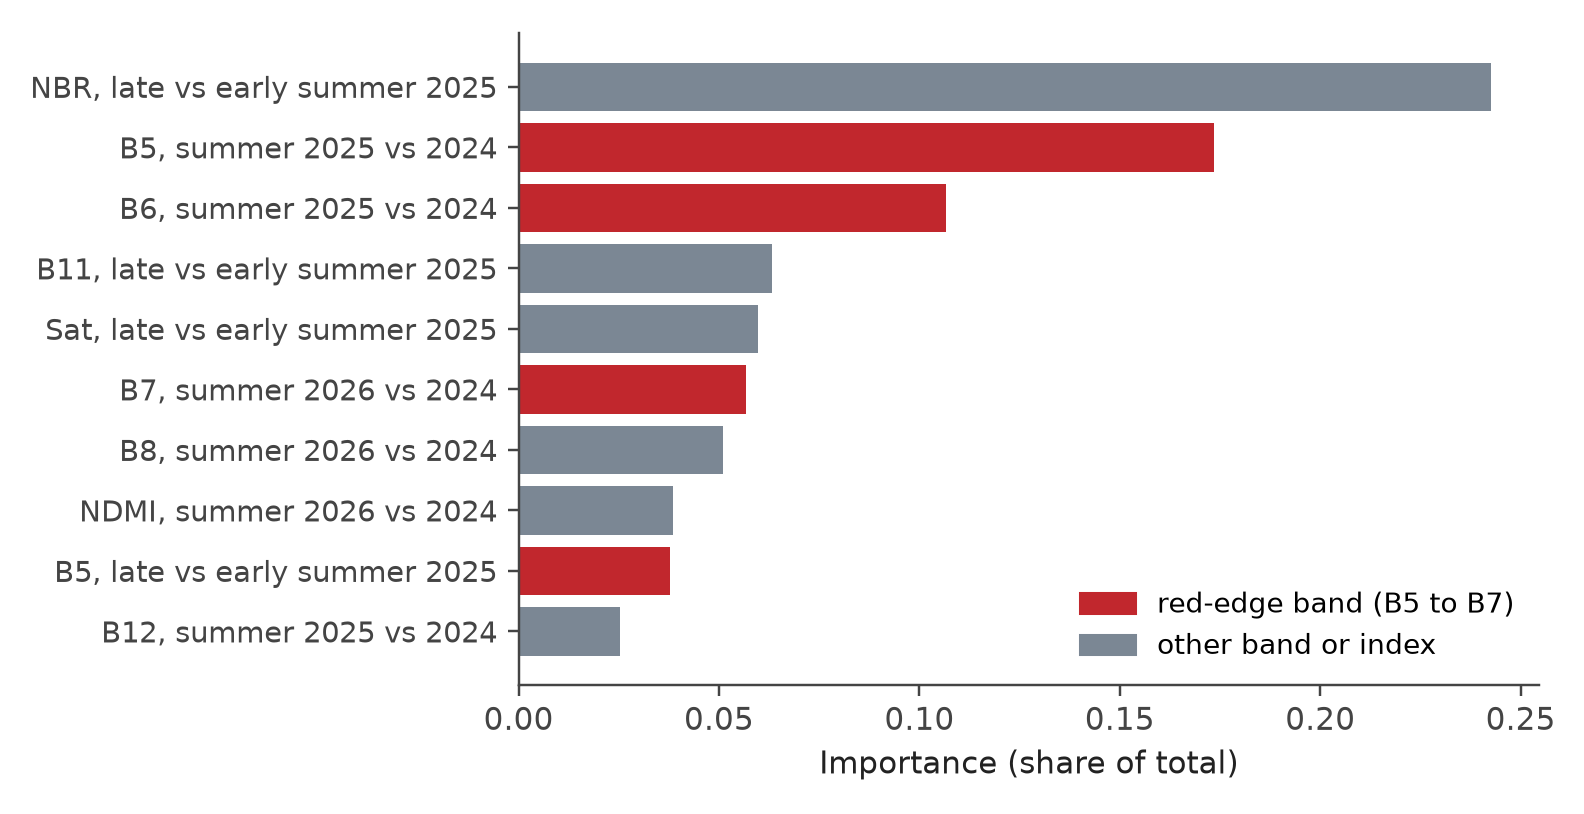
\includegraphics[width=0.78\linewidth]{fig_beetle_importance.png}
\captionof{figure}{The ten measures gradient boosting relies on most. Each is the change in a band or index between two periods.}\label{fig:importance}
\end{minipage}
\item \textbf{The damage is not clearly visible a year later.} Summer 2026 against summer 2024 shows no clear relationship with the survey, either because the heather recovered or because damaged heather was burnt or cut in 2025/26 and is masked out.
\end{itemize}

\subsection{How far the estimate can be trusted}

The model never sees the moor it predicts, the line converting probability to a proportion is fitted on held-out predictions, and all measures are image changes, not survey scores. Two further tests look for optimism that the design cannot rule out (\appref{app:beetle-leakage}):
\begin{itemize}
\item \textbf{Choosing the model after the fact.} Six models were compared (\appref{app:beetle-models}). When the model is chosen inside each fold from the training moors only, the combined estimate scores 0.105 against 0.098, so the choice adds very little.
\item \textbf{Similar neighbouring moors.} When a whole region is hidden from training, gradient boosting alone does markedly worse (0.22 against 0.12 on those 8 count areas), but the combined estimate holds up (0.07, close to the rule's 0.08) because the rule needs no training. This is why the combined estimate, not the model alone, is reported.
\end{itemize}

\subsection{Imagery where satellite and survey differ most}

\begin{figure}[htbp]
\centering
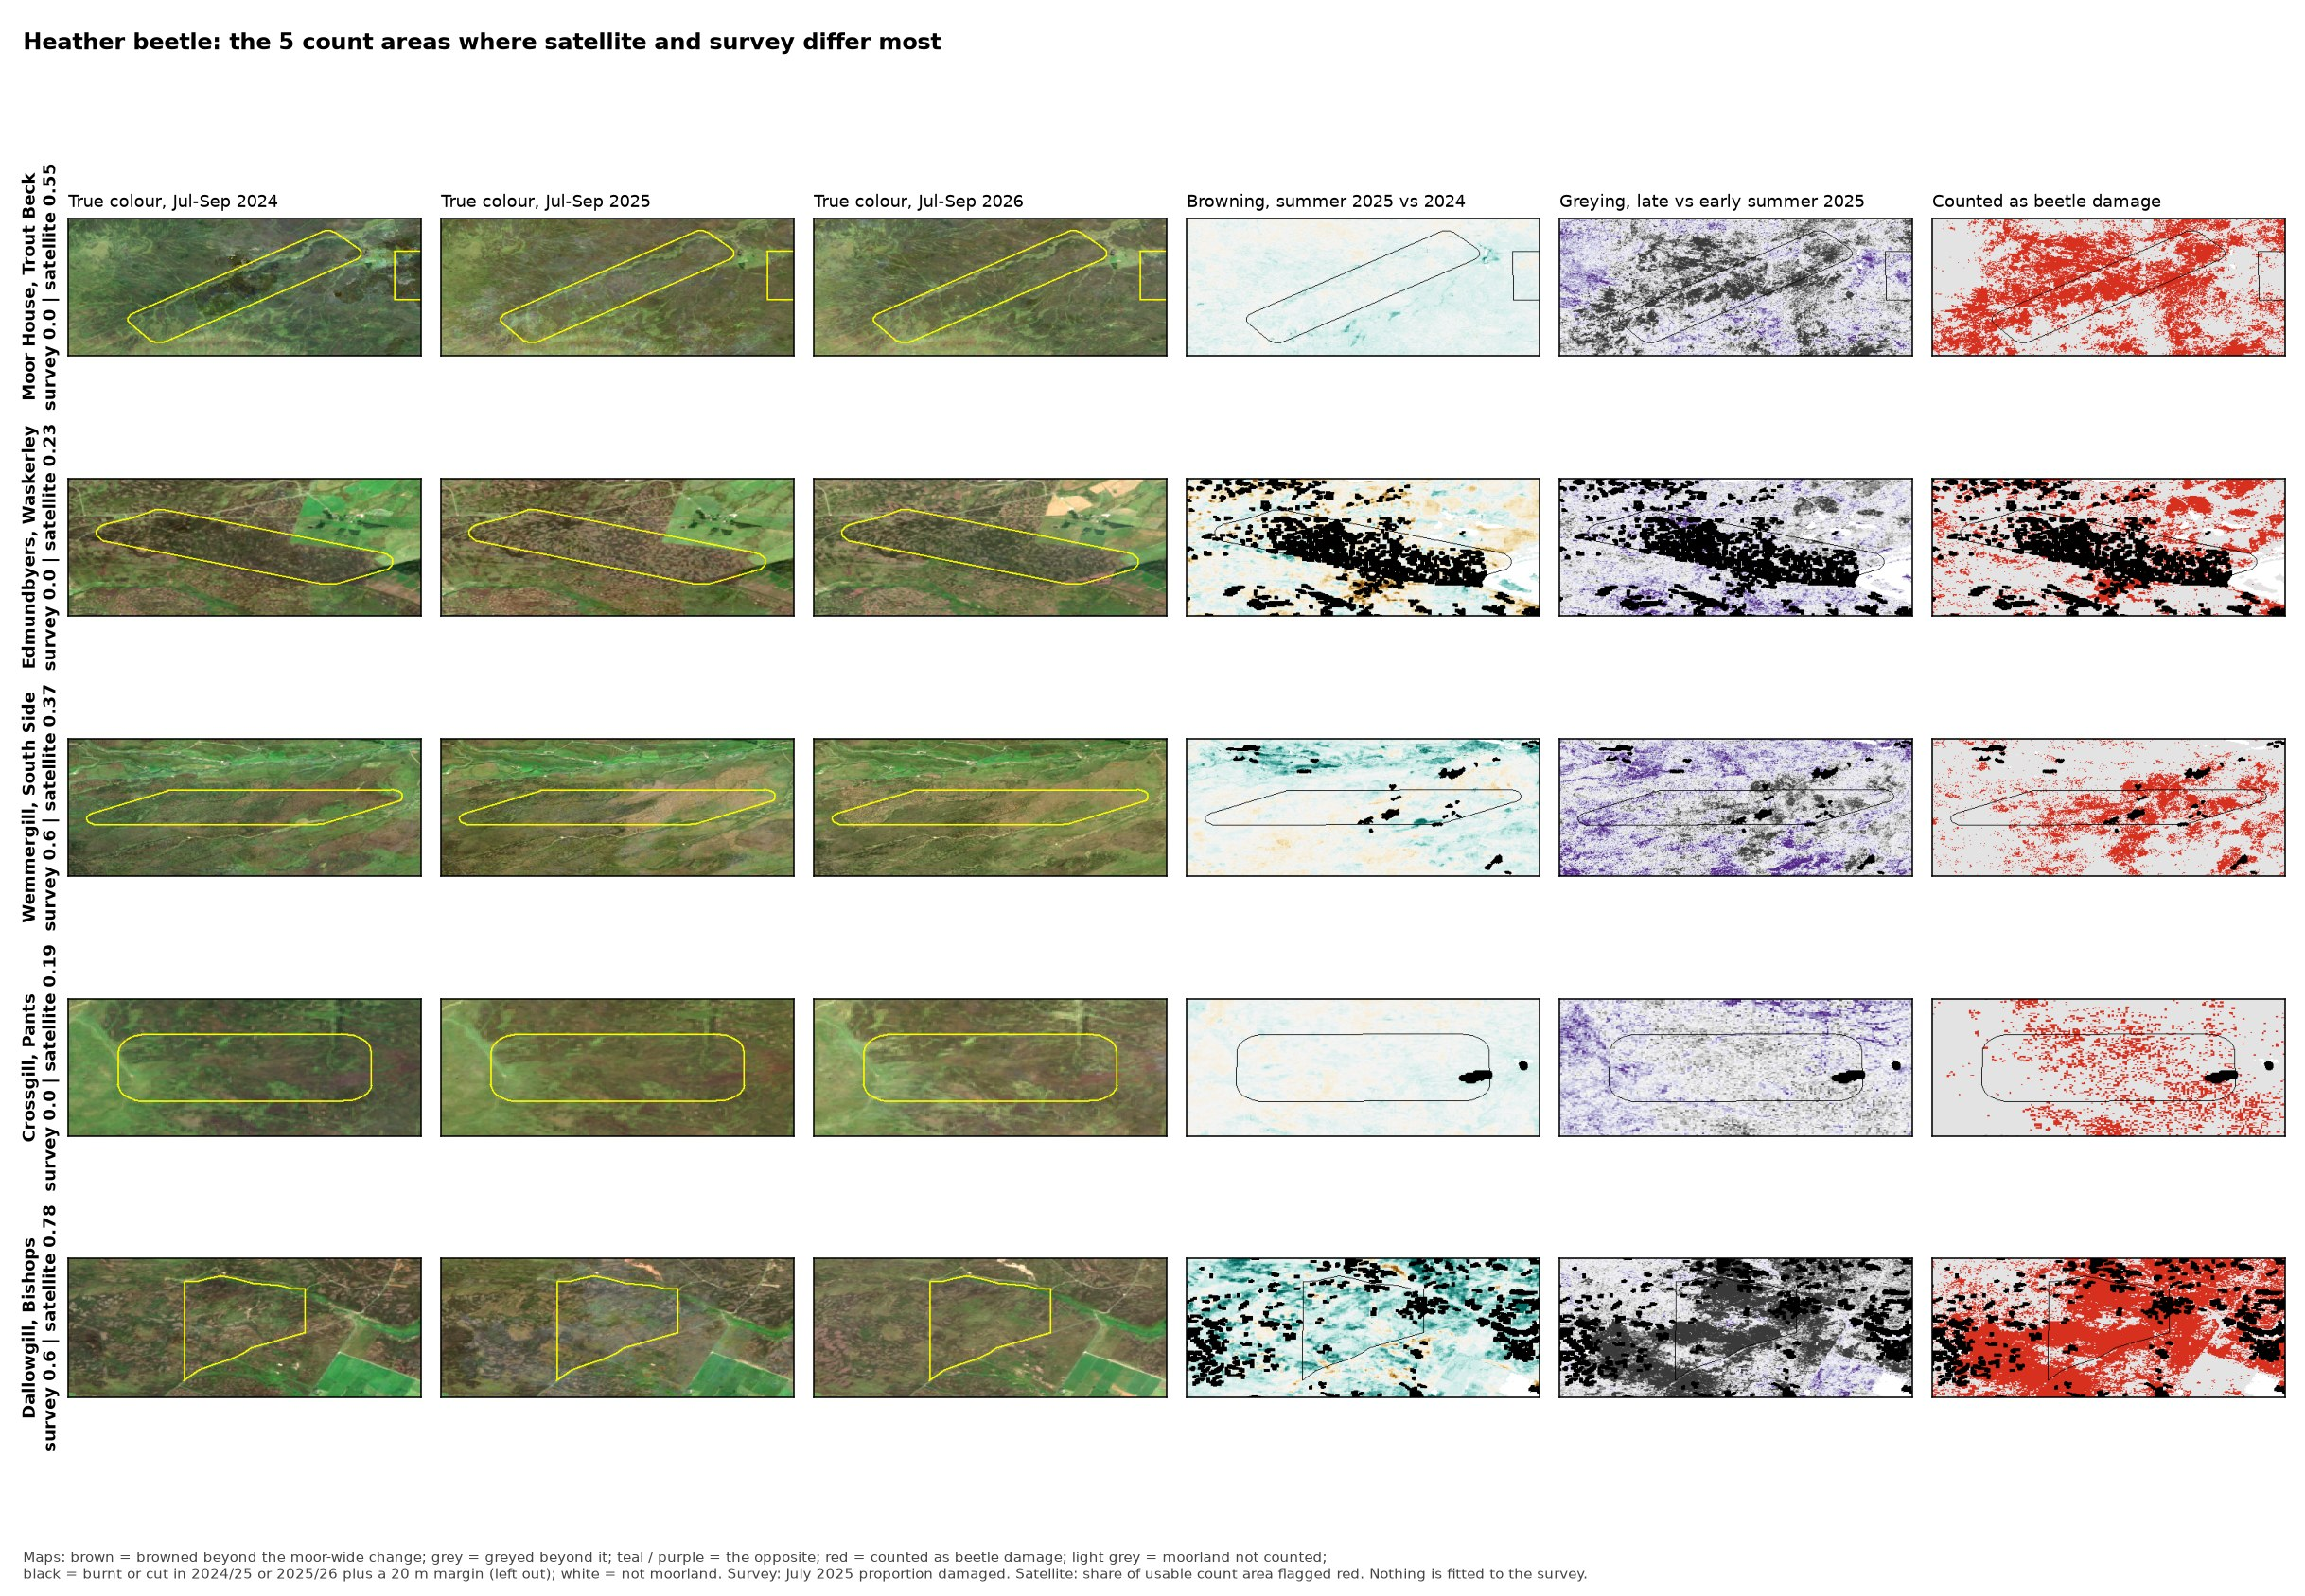
\includegraphics[width=\linewidth]{fig_evidence_disagree.jpg}
\caption{The five count areas where the rule-based estimate and the survey differ most. Left to right: true colour 2024, 2025 and 2026; browning; greying; pixels counted as damage (red). Black is burnt or cut ground plus a 20~m margin.}\label{fig:evidence}
\end{figure}

At 10~m the true-colour images show the damage only faintly; the change maps say more (\figref{fig:evidence}). At these count areas the imagery mostly supports the survey:
\begin{itemize}
\item \textbf{Moor House, Trout Beck} (survey 0, rule 0.55, combined 0.30): the greying covers the whole bog, inside and outside the count area. It does not look like beetle damage, and gradient boosting discounts it.
\item \textbf{Edmundbyers, Waskerley} (survey 0, rule 0.23): heavily burnt in 2024/25; the remaining flags sit around the burns.
\item \textbf{Wemmergill, South Side} (survey 0.6, rule 0.37, combined 0.24): some flagged patches inside the count area, but fewer than the survey suggests. Field photos would settle it.
\end{itemize}

\FloatBarrier
% ================================================================ 7 discussion
\section{Discussion}\label{sec:discussion}

\subsection{Total management is the right measure}

Since 2021 the question for grouse moors is no longer only how much is burnt, but how much is managed. Burning and cutting look alike at 10~m and happen in the same season, so the satellite measures their sum. That is a limitation for a study of burning, but it is the quantity that matters for grouse and for habitat structure. Read this way, the steady total after 2021 and the 2024/25 peak both fit what managers report.

\subsection{Agreement with published work}

The regional ordering and the North York Moors level match \citet{shewring2024}, derived independently with a different method. The higher North Pennines figure and the absence of a post-2021 fall are both expected when cutting is included. A direct test would compare the two methods on the same ground for 2017/18 to 2021/22, burning only, on moors where cutting is rare.

\subsection{Using the results with grouse counts}

Because management is sporadic, a count area's figure in a single season can be large or zero. Every season is valid, and season-specific values can be related to the following summer's count. For a measure of management intensity, the mean over several seasons is more stable. The results file holds both: hectares and percentage for each count area in each season.

\subsection{Limits and how to address them}

\begin{table}[H]
\centering
\caption{Limits of the analysis and how to address them.}\label{tab:limits}
\footnotesize
\begin{tabularx}{\linewidth}{>{\raggedright\arraybackslash}p{0.24\linewidth}>{\raggedright\arraybackslash}p{0.33\linewidth}L}
\toprule
Limit & Effect & How to address it \\
\midrule
Cuts below 0.1~ha & Small cuts are missed; Crossgill and Wemmergill read low & Aerial imagery (APGB, 25 or 50~cm) or PlanetScope (3~m) \\
No accuracy figure yet & The threshold is calibrated and stable, but not validated & Ground truth at 15 to 20 known burn and cut sites \\
Burning and cutting together & Their shares cannot be reported separately & Aerial imagery: cuts have straight edges and tracks \\
Management of dead heather & Likely under-counted in beetle years & Damage records from 2024; ground truth in damaged areas \\
Uneven image supply & A few count-area seasons rest on very few clear images (Grinton 2024/25) & Flagged in the results; PlanetScope would fill gaps \\
Beetle model: one year, 22 count areas & Differences of 0.01 to 0.02 between methods are within chance & A second survey year; a few hundred hand-checked patches \\
\bottomrule
\end{tabularx}
\end{table}

% ================================================================ 8 conclusions
\section{Conclusions and recommendations}\label{sec:conclusions}

Sentinel-2 records total heather management on red grouse count areas consistently from season to season. About 4\% of the count area is burnt or cut in an average season, with sporadic heavy seasons on individual count areas, a higher level on the North York Moors, a steady total after the 2021 regulation and a peak in 2024/25 during the heather beetle outbreak. These patterns hold under every test applied. PW's review changed how the results are read and improved the method; of the individual changes, the smaller minimum patch mattered most. Sentinel-2 can also estimate heather beetle damage to within about 0.1 of a field survey.

\textbf{Immediate}
\begin{enumerate}
\item \textbf{Ground-truth the method.} Identify 15 to 20 sites where burning or cutting is known (estate records or field visits), digitise them and run the detection against them. This gives an accuracy figure and is the most important next step.
\item \textbf{Beetle damage evidence:} field photos from the July 2025 survey (ideally with locations), any damage scores from 2024, and a note of how the scores were estimated.
\item \textbf{Check two single results} with the estates: the 40~ha block at Pikestone Fell in 2022/23 (possibly a wildfire), and Geltsdale's detections (1.0\% a year).
\end{enumerate}

\textbf{Next}
\begin{enumerate}[resume]
\item \textbf{Aerial imagery} (APGB, 25 or 50~cm, colour infrared). At this resolution cuts and burns can be told apart by their shape, and small cuts become visible. Check whether GWCT already has access.
\item \textbf{Develop the beetle damage model.} A second survey year would test it on new data, and a few hundred hand-checked patches (beetle-brown, beetle-grey, burnt, cut, healthy) would let it map damage pixel by pixel. Test any version by holding out one moor at a time.
\item \textbf{PlanetScope} (3~m, near-daily), free under Planet's Education and Research programme, is the intermediate option between Sentinel-2 and aerial imagery.
\item \textbf{Replace the fixed threshold with a supervised classifier} once ground-truth data exist.
\end{enumerate}

% ================================================================ references
\begin{thebibliography}{99}
\addcontentsline{toc}{section}{References}
\bibitem[Drusch et~al.(2012)]{drusch2012} Drusch, M., Del Bello, U., Carlier, S. et~al. (2012) Sentinel-2: ESA's optical high-resolution mission for GMES operational services. \emph{Remote Sensing of Environment}, 120, 25--36.
\bibitem[Friedman(2001)]{friedman2001} Friedman, J.H. (2001) Greedy function approximation: a gradient boosting machine. \emph{Annals of Statistics}, 29, 1189--1232.
\bibitem[Gorelick et~al.(2017)]{gorelick2017} Gorelick, N., Hancher, M., Dixon, M., Ilyushchenko, S., Thau, D. \& Moore, R. (2017) Google Earth Engine: planetary-scale geospatial analysis for everyone. \emph{Remote Sensing of Environment}, 202, 18--27.
\bibitem[Key and Benson(2006)]{key2006} Key, C.H. \& Benson, N.C. (2006) Landscape assessment: sampling and analysis methods. In \emph{FIREMON: Fire Effects Monitoring and Inventory System}. USDA Forest Service General Technical Report RMRS-GTR-164-CD.
\bibitem[Pedregosa et~al.(2011)]{pedregosa2011} Pedregosa, F., Varoquaux, G., Gramfort, A. et~al. (2011) Scikit-learn: machine learning in Python. \emph{Journal of Machine Learning Research}, 12, 2825--2830.
\bibitem[Roberts et~al.(2017)]{roberts2017} Roberts, D.R., Bahn, V., Ciuti, S. et~al. (2017) Cross-validation strategies for data with temporal, spatial, hierarchical, or phylogenetic structure. \emph{Ecography}, 40, 913--929.
\bibitem[Shewring et~al.(2024)]{shewring2024} Shewring, M.P., Wilkinson, N.I., Teuten, E.L., Buchanan, G.M., Thompson, P. \& Douglas, D.J.T. (2024) Annual extent of prescribed burning on moorland in Great Britain and overlap with ecosystem services. \emph{Remote Sensing in Ecology and Conservation}. doi:10.1002/rse2.389.
\bibitem[{The Heather and Grass etc.\ Burning (England) Regulations}(2021)]{regs2021} The Heather and Grass etc.\ Burning (England) Regulations 2021. SI 2021/158.
\bibitem[Zanaga et~al.(2022)]{zanaga2022} Zanaga, D., Van De Kerchove, R., Daems, D. et~al. (2022) ESA WorldCover 10~m 2021 v200. Zenodo. doi:10.5281/zenodo.7254221.
\end{thebibliography}

% ================================================================ appendices
\clearpage
\appendix
\addtocontents{toc}{\protect\vspace{0.6em}{\sffamily\bfseries\color{accent}Appendices}\protect\par\protect\setcounter{tocdepth}{1}}
\floatplacement{figure}{H}
\floatplacement{table}{H}
\renewcommand{\thesection}{\Alph{section}}

\section{Formulae}\label{app:formulae}

Notation: $\rho_k(x,t)$ is the surface reflectance of Sentinel-2 band $k$ at pixel $x$ on date $t$ (digital numbers divided by 10,000). $\mathbf{1}[\cdot]$ is 1 when the condition holds and 0 otherwise.

\subsection{Indices}
\begin{gather*}
\mathrm{NBR} = \frac{\rho_{B8}-\rho_{B12}}{\rho_{B8}+\rho_{B12}}, \qquad \mathrm{NDVI} = \frac{\rho_{B8}-\rho_{B4}}{\rho_{B8}+\rho_{B4}}, \qquad \mathrm{NDMI} = \frac{\rho_{B8}-\rho_{B11}}{\rho_{B8}+\rho_{B11}} \\[4pt]
\text{Brightness} = \tfrac{1}{3}\left(\rho_{B2}+\rho_{B3}+\rho_{B4}\right), \qquad S = \frac{\max(\rho_{B2},\rho_{B3},\rho_{B4})-\min(\rho_{B2},\rho_{B3},\rho_{B4})}{\max(\rho_{B2},\rho_{B3},\rho_{B4})}
\end{gather*}
The colour saturation $S$ is 0 for a perfectly grey surface and rises with colour.

\subsection{Composites}
A scene is clear at $x$ if its s2cloudless cloud probability is below 40\% and its scene classification is not cloud shadow, cloud (medium or high), cirrus or snow (classes 3, 8, 9, 10, 11). For any index $I$ and window $W$:
\[
I_W(x) = \operatorname*{median}_{t \in W,\ \text{clear at } x} I(x,t)
\]

\subsection{Change and seasonal correction}
For season $s$, with the before window $W_b$ (1 July to 30 September) and the after window $W_a$ (16 April to 30 June):
\begin{gather*}
\mathrm{dNBR}_s(x) = \mathrm{NBR}_{W_b}(x) - \mathrm{NBR}_{W_a}(x) \\
c_s = \operatorname*{median}_{x \in M} \mathrm{dNBR}_s(x), \qquad \mathrm{dNBR}^{*}_s(x) = \mathrm{dNBR}_s(x) - c_s
\end{gather*}
where $M$ is the moorland in all count areas, sampled at 100~m. The threshold check reports $p_{95,s}$, the 95th percentile of $\mathrm{dNBR}^{*}_s$ over $M$.

\subsection{Detection}
\[
r_s(x) = \mathbf{1}\!\left[\mathrm{dNBR}^{*}_s(x) > \tau\right]\cdot \mathbf{1}\!\left[\mathrm{NDVI}_{W_b}(x) > 0.3\right]\cdot \mathbf{1}\!\left[x \in M\right], \qquad \tau = 0.17
\]
\[
m_s(x) = r_s(x)\cdot \mathbf{1}\!\left[\,|P_s(x)| \ge 10\,\right]
\]
where $P_s(x)$ is the patch of pixels with $r_s = 1$ connected to $x$ through any of its eight neighbours. Ten 10~m pixels are 0.1~ha.

\subsection{Areas and percentages}
For count area $a$ with area $A_a$, and pixel area $\omega(x)$ weighted by the fraction of the pixel inside $a$:
\[
H_{a,s} = \sum_{x \in a} m_s(x)\,\omega(x), \qquad \%_{a,s} = 100\,\frac{H_{a,s}}{A_a}
\]
For a group $G$ of count areas (a moor, a region, or all) over seasons $s = 1,\dots,9$, the mean annual percentage is area-weighted:
\[
\%_G = 100\,\frac{\sum_{a\in G}\sum_s H_{a,s}}{\sum_{a\in G}\sum_s A_a}
\]

\subsection{Beetle damage: rule-based estimate}
\begin{gather*}
\Delta\mathrm{NBR}(x) = \mathrm{NBR}_{\text{Jul to Sep 2025}}(x) - \mathrm{NBR}_{\text{Jul to Sep 2024}}(x) \\
\Delta S(x) = S_{\text{Jul to Sep 2025}}(x) - S_{\text{16 Apr to 30 Jun 2025}}(x)
\end{gather*}
$U$ is the usable ground: moorland, excluding pixels within 20~m of ground detected as burnt or cut in 2024/25 or 2025/26. Each change is centred on its median over $U$ in all count areas (sampled at 20~m):
\[
\Delta\mathrm{NBR}^{*}(x) = \Delta\mathrm{NBR}(x) - \operatorname*{median}_{U}\Delta\mathrm{NBR}, \qquad \Delta S^{*}(x) = \Delta S(x) - \operatorname*{median}_{U}\Delta S
\]
\[
f(x) = \mathbf{1}\!\left[\Delta\mathrm{NBR}^{*}(x) < -0.10 \;\text{ or }\; \Delta S^{*}(x) < -0.05\right], \qquad R_a = \frac{1}{|a\cap U|}\sum_{x\in a\cap U} f(x)
\]

\subsection{Beetle damage: gradient boosting}
\textbf{Labels from the survey.} With $d_a$ the surveyed damage of count area $a$, each sampled pixel $x$ in $a$ gets
\[
y_x = \begin{cases}0 & d_a = 0\\ 1 & d_a \ge 0.5\\ \text{no label} & \text{otherwise.}\end{cases}
\]
\textbf{Measures.} $z_x$ holds 45 changes: 15 measures (bands B2, B3, B4, B5, B6, B7, B8, B8A, B11, B12; NBR, NDVI, NDMI, $S$, brightness) for each of three comparisons (summer 2025 minus summer 2024; late minus early summer 2025; summer 2026 minus summer 2024).

\textbf{Model.} Gradient boosting \citep{friedman2001}, as implemented in scikit-learn \citep{pedregosa2011}, builds an additive score from $M$ small regression trees $h_m$ (depth 3):
\[
F_M(z) = F_0 + \nu\sum_{m=1}^{M} h_m(z), \qquad p(z) = \frac{1}{1+e^{-F_M(z)}}
\]
Each tree is fitted, on a random 80\% of the labelled pixels, to the negative gradient of the log-loss
\[
L = -\sum_x \left[\,y_x \log p(z_x) + (1-y_x)\log\!\left(1-p(z_x)\right)\right]
\]
with learning rate $\nu = 0.05$ and $M = 150$ trees.

\textbf{From pixels to a count area.} The mean probability $\bar p_a = \frac{1}{n_a}\sum_{x\in a} p(z_x)$ is mapped to a proportion with a straight line fitted by least squares on the training count areas, using out-of-fold probabilities:
\[
\hat d_a = \min\!\left(1,\ \max\!\left(0,\ \alpha + \beta\,\bar p_a\right)\right)
\]
\textbf{Combined estimate.} $\hat c_a = \tfrac{1}{2}\left(R_a + \hat d_a\right)$.

\subsection{Evaluation}
\textbf{Leave-one-moor-out.} For each moor $m$, the model and its calibration line are fitted using only the other moors' pixels and survey scores; $\hat c_a$ is then computed for the count areas of $m$. The moor-wide medians above use imagery from all count areas but no survey scores.
\[
\text{Typical difference} = \frac{1}{n}\sum_{a=1}^{n}\left|\hat c_a - d_a\right|, \qquad \text{Within } k = \#\left\{a : \left|\hat c_a - d_a\right| \le k\right\}
\]
\textbf{Rank agreement} is Spearman's $\rho$: the Pearson correlation of the ranks of $\hat c_a$ and $d_a$.

\textbf{Paired bootstrap.} For $b = 1,\dots,5000$, draw $n$ count areas with replacement and compute $\Delta_b = \mathrm{TD}^{\text{model}}_b - \mathrm{TD}^{\text{rule}}_b$, the difference in typical difference on that sample; the 90\% interval is the 5th to 95th percentile of $\Delta_b$.

\textbf{Region-only benchmark.} $\hat d_a$ is the mean of $d$ over the other moors in the same GWCT region.

\textbf{Nested model choice.} For each held-out moor $m$, the training moors are split into five groups. Each candidate model's combined estimate is scored by holding out each group in turn; the model with the lowest typical difference is refitted on all training moors, and it alone predicts $m$.

\textbf{Region hold-out.} As leave-one-moor-out, but every moor in one GWCT region is held out together (North York Moors; southern Dales). The northern Dales region cannot be held out: it contains every count area the survey scored 0.

\clearpage
\section{Threshold sensitivity}\label{app:thresholds}

\begin{table}[H]
\centering
\caption{Main results at four detection thresholds.}\label{tab:thresholds}
\footnotesize
\setlength{\tabcolsep}{4.5pt}
\begin{threeparttable}
\begin{tabular}{lrrrrrrr}
\toprule
Threshold & \makecell[r]{Total\\vs 0.17} & \makecell[r]{Season\\order\textsuperscript{a}} & \makecell[r]{Moor\\order\textsuperscript{a}} & \makecell[r]{NYM /\\NP} & \makecell[r]{After /\\before 2021} & \makecell[r]{Moor\\House \%} & \makecell[r]{Geltsdale\\\%} \\
\midrule
0.13 & +61\% & 0.97 & 0.98 & 1.64 & 1.03 & 0.65 & 4.5 \\
0.15 & +25\% & 0.98 & 0.99 & 1.72 & 1.00 & 0.23 & 2.0 \\
\textbf{0.17} & main run & 1.00 & 1.00 & 1.75 & 0.98 & 0.08 & 1.0 \\
0.19 & $-$20\% & 0.93 & 1.00 & 1.78 & 0.97 & 0.02 & 0.6 \\
\bottomrule
\end{tabular}

\begin{tablenotes}\footnotesize
\item[a] Rank correlation with the 0.17 results. NYM / NP: North York Moors against North Pennines, mean annual percentage. After / before 2021: mean of 2021/22 to 2023/24 against 2017/18 to 2020/21.
\end{tablenotes}
\end{threeparttable}
\end{table}

Lowering the threshold barely changes the after/before 2021 ratio (0.97 to 1.03), so there is no sign that faint cut scars, which a lower threshold would pick up, cluster after the regulation. At 0.13 the reserves register clearly (Moor House 0.65\%, Geltsdale 4.5\% a year), which marks 0.13 as too permissive. At 0.19 Geltsdale falls to 0.55\%.

\section{Further results on heather beetle damage}\label{app:beetle}

\subsection{Earlier attempts}\label{app:beetle-early}

\begin{itemize}
\item \textbf{Browning alone} (the share of each count area whose NBR fell from summer 2024 to summer 2025): typical difference 0.27, rank agreement 0.60. The whole area browned in the dry summer of 2025, so the moor-wide change has to be removed.
\item \textbf{Rule-based estimate without the 20~m margin} around burnt and cut ground: typical difference 0.13. Edges of fresh burns were being counted as damage.
\item \textbf{A heather mask from seasonal greenness} (heather stays green in winter): typical difference 0.15, worse than without it. WorldCover has no heather class in these count areas, so no better mask was available.
\item \textbf{Calibrating the rule-based estimate} with a straight line fitted on the other moors: typical difference 0.125, no better than the uncalibrated share (0.123), so the rule is used as it stands.
\item \textbf{A random forest on its own:} typical difference 0.13 as a classifier of healthy and damaged pixels, and 0.16 predicting each pixel's survey score directly. Averaged with the rule it reaches 0.11 (\appref{app:beetle-models}).
\end{itemize}

\subsection{Six models compared}\label{app:beetle-models}

\begin{table}[H]
\centering
\caption{Six models for Step 2, alone and averaged with the rule-based estimate. 22 count areas, leave-one-moor-out. The interval is the paired-bootstrap 90\% interval for the change in typical difference against the rule alone; negative is better.}\label{tab:models}
\scriptsize
\setlength{\tabcolsep}{3.5pt}
\begin{tabular}{lrrrrrrrl}
\toprule
& \multicolumn{3}{c}{Model alone} & \multicolumn{5}{c}{Averaged with the rule} \\ \cmidrule(lr){2-4}\cmidrule(lr){5-9}Model & \makecell[r]{Typical\\diff.} & \makecell[r]{Within\\0.1} & \makecell[r]{Rank\\$\rho$} & \makecell[r]{Typical\\diff.} & \makecell[r]{Within\\0.1} & \makecell[r]{Within\\0.2} & \makecell[r]{Rank\\$\rho$} & \makecell[l]{90\% interval\\vs rule} \\
\midrule
Rule-based estimate only & 0.122 & 12 & 0.81 &  &  &  &  &  \\
\midrule
\textbf{Gradient boosting (classic)} & 0.118 & 10 & 0.79 & 0.098 & 15 & 19 & 0.88 & $-$0.053 to $+$0.003 \\
Gradient boosting (LightGBM style) & 0.122 & 10 & 0.78 & 0.101 & 15 & 20 & 0.87 & $-$0.049 to $+$0.006 \\
Support vector machine & 0.124 & 11 & 0.78 & 0.102 & 15 & 20 & 0.86 & $-$0.049 to $+$0.008 \\
Random forest & 0.141 & 12 & 0.78 & 0.109 & 14 & 19 & 0.86 & $-$0.043 to $+$0.013 \\
Logistic regression & 0.151 & 9 & 0.72 & 0.109 & 13 & 19 & 0.84 & $-$0.043 to $+$0.018 \\
Extra trees & 0.161 & 9 & 0.71 & 0.118 & 11 & 19 & 0.83 & $-$0.032 to $+$0.022 \\
\bottomrule
\end{tabular}

\end{table}

All six models improve on the rule when averaged with it, with typical differences of 0.10 to 0.12 (\tabref{tab:models}). Classic gradient boosting is best (0.098) and is used in the report. Every 90\% interval includes zero: with 22 count areas the gains are consistent across models but individually within chance. More and better labels will matter more than the choice of algorithm. The models were fitted with scikit-learn \citep{pedregosa2011}: gradient boosting with 150 trees of depth 3, learning rate 0.05 and 80\% subsampling, settings fixed in advance.

\subsection{Checks for data leakage}\label{app:beetle-leakage}

Leakage means information about the answer reaching the model, which makes results look better than they will be on new data. The burning and cutting analysis fits nothing to outcomes, so this applies only to the beetle model.

\begin{table}[H]
\centering
\caption{Possible sources of leakage and how they are handled.}\label{tab:leakage}
\footnotesize
\begin{tabularx}{\linewidth}{>{\raggedright\arraybackslash}p{0.36\linewidth}L}
\toprule
Possible leak & How it is handled \\
\midrule
A moor's own pixels or survey score used to predict it & Never: every estimate comes from a model trained without that moor \\
Calibration fitted on the model's own training fit & The line uses out-of-fold probabilities, split by moor \\
Measures built from survey scores & All measures are image changes \\
Settings tuned on the test results & Model settings were fixed in advance \\
Moor-wide reference includes the held-out moor & Imagery only, no survey scores; one moor barely moves a median over 4,000~ha \\
Choosing the best of six models on the same data & Nested test: 0.105 against 0.098; classic gradient boosting chosen in 9 of 15 folds \\
Similar neighbouring moors in training & Region hold-out (\tabref{tab:region}) \\
\bottomrule
\end{tabularx}
\end{table}

\begin{table}[H]
\centering
\caption{Region hold-out: typical difference on the 8 count areas of the North York Moors and the southern Dales.}\label{tab:region}
\small
\begin{tabular}{lcc}
\toprule
Estimate & Alone & Averaged with the rule \\
\midrule
Rule-based estimate & 0.075 & \\
Gradient boosting, one moor held out & 0.124 & 0.059 \\
Gradient boosting, whole region held out & 0.215 & 0.072 \\
\bottomrule
\end{tabular}
\end{table}

Gradient boosting alone relies partly on having seen similar moors nearby; averaged with the rule it holds up when a whole region is unseen (\tabref{tab:region}). The flagging cut-offs and model settings were fixed in advance, but greying as a measure and the decision to average were settled while looking at the same 22 count areas. A second survey year is the clean test.

\subsection{Estimates for every count area}\label{app:beetle-areas}

\begin{table}[H]
\centering
\caption{Surveyed damage and satellite estimates by count area, each moor predicted without its own data. Grinton, Long Gill (survey 0.5) had too few clear images and is not estimated.}\label{tab:beetle-areas}
\footnotesize
\begin{tabular}{lrrrrr}
\toprule
Count area & Survey & Rule & \makecell[r]{Gradient\\boosting} & Combined & Difference \\
\midrule
\multicolumn{6}{l}{\textit{Northern Dales}} \\
Bollihope, Pikestone Fell & 0.0 & 0.14 & 0.13 & \textbf{0.13} & +0.13 \\
Crossgill, Dowks & 0.0 & 0.02 & 0.17 & \textbf{0.09} & +0.09 \\
Crossgill, Pants & 0.0 & 0.19 & 0.14 & \textbf{0.16} & +0.16 \\
Edmundbyers, Waskerley & 0.0 & 0.23 & 0.17 & \textbf{0.20} & +0.20 \\
Geltsdale, Middle & 0.0 & 0.13 & 0.00 & \textbf{0.07} & +0.07 \\
Moor House, Trout Beck & 0.0 & 0.55 & 0.05 & \textbf{0.30} & +0.30 \\
Moor House, Behind House & 0.0 & 0.10 & 0.01 & \textbf{0.05} & +0.05 \\
Stags Fell, Beacon & 0.0 & 0.08 & 0.00 & \textbf{0.04} & +0.04 \\
Crossgill, Greencastles & 0.1 & 0.03 & 0.24 & \textbf{0.14} & +0.04 \\
Wemmergill, Close House & 0.1 & 0.20 & 0.01 & \textbf{0.11} & +0.01 \\
Bollihope, Catterick & 0.3 & 0.41 & 0.47 & \textbf{0.44} & +0.14 \\
Eggleston, Ever Rigg & 0.3 & 0.31 & 0.29 & \textbf{0.30} & +0.00 \\
Eggleston, Blackton & 0.3 & 0.43 & 0.34 & \textbf{0.38} & +0.08 \\
Wemmergill, South Side & 0.6 & 0.37 & 0.11 & \textbf{0.24} & $-$0.36 \\
\midrule
\multicolumn{6}{l}{\textit{North York Moors}} \\
Danby, Low Moor & 0.5 & 0.51 & 0.61 & \textbf{0.56} & +0.06 \\
Westerdale, Tank & 0.5 & 0.54 & 0.65 & \textbf{0.59} & +0.09 \\
Rosedale, Pits & 0.6 & 0.69 & 0.66 & \textbf{0.67} & +0.07 \\
Danby, Glaisdale & 0.7 & 0.76 & 0.65 & \textbf{0.70} & +0.00 \\
Snilesworth, Lodge & 0.8 & 0.92 & 0.57 & \textbf{0.74} & $-$0.06 \\
\midrule
\multicolumn{6}{l}{\textit{Southern Dales and Peak}} \\
Ramsgill, Raygill & 0.2 & 0.22 & 0.39 & \textbf{0.30} & +0.10 \\
Dallowgill, Bishops & 0.6 & 0.78 & 0.53 & \textbf{0.66} & +0.06 \\
Swinton, Potts & 0.7 & 0.78 & 0.56 & \textbf{0.67} & $-$0.03 \\
\bottomrule
\end{tabular}

\end{table}

Where the survey found little or no damage (0 to 0.1), the combined estimate runs about 0.11 high on average. Survey scores are estimates in tenths, so agreement much closer than 0.1 cannot be expected.

\begin{figure}[H]
\centering
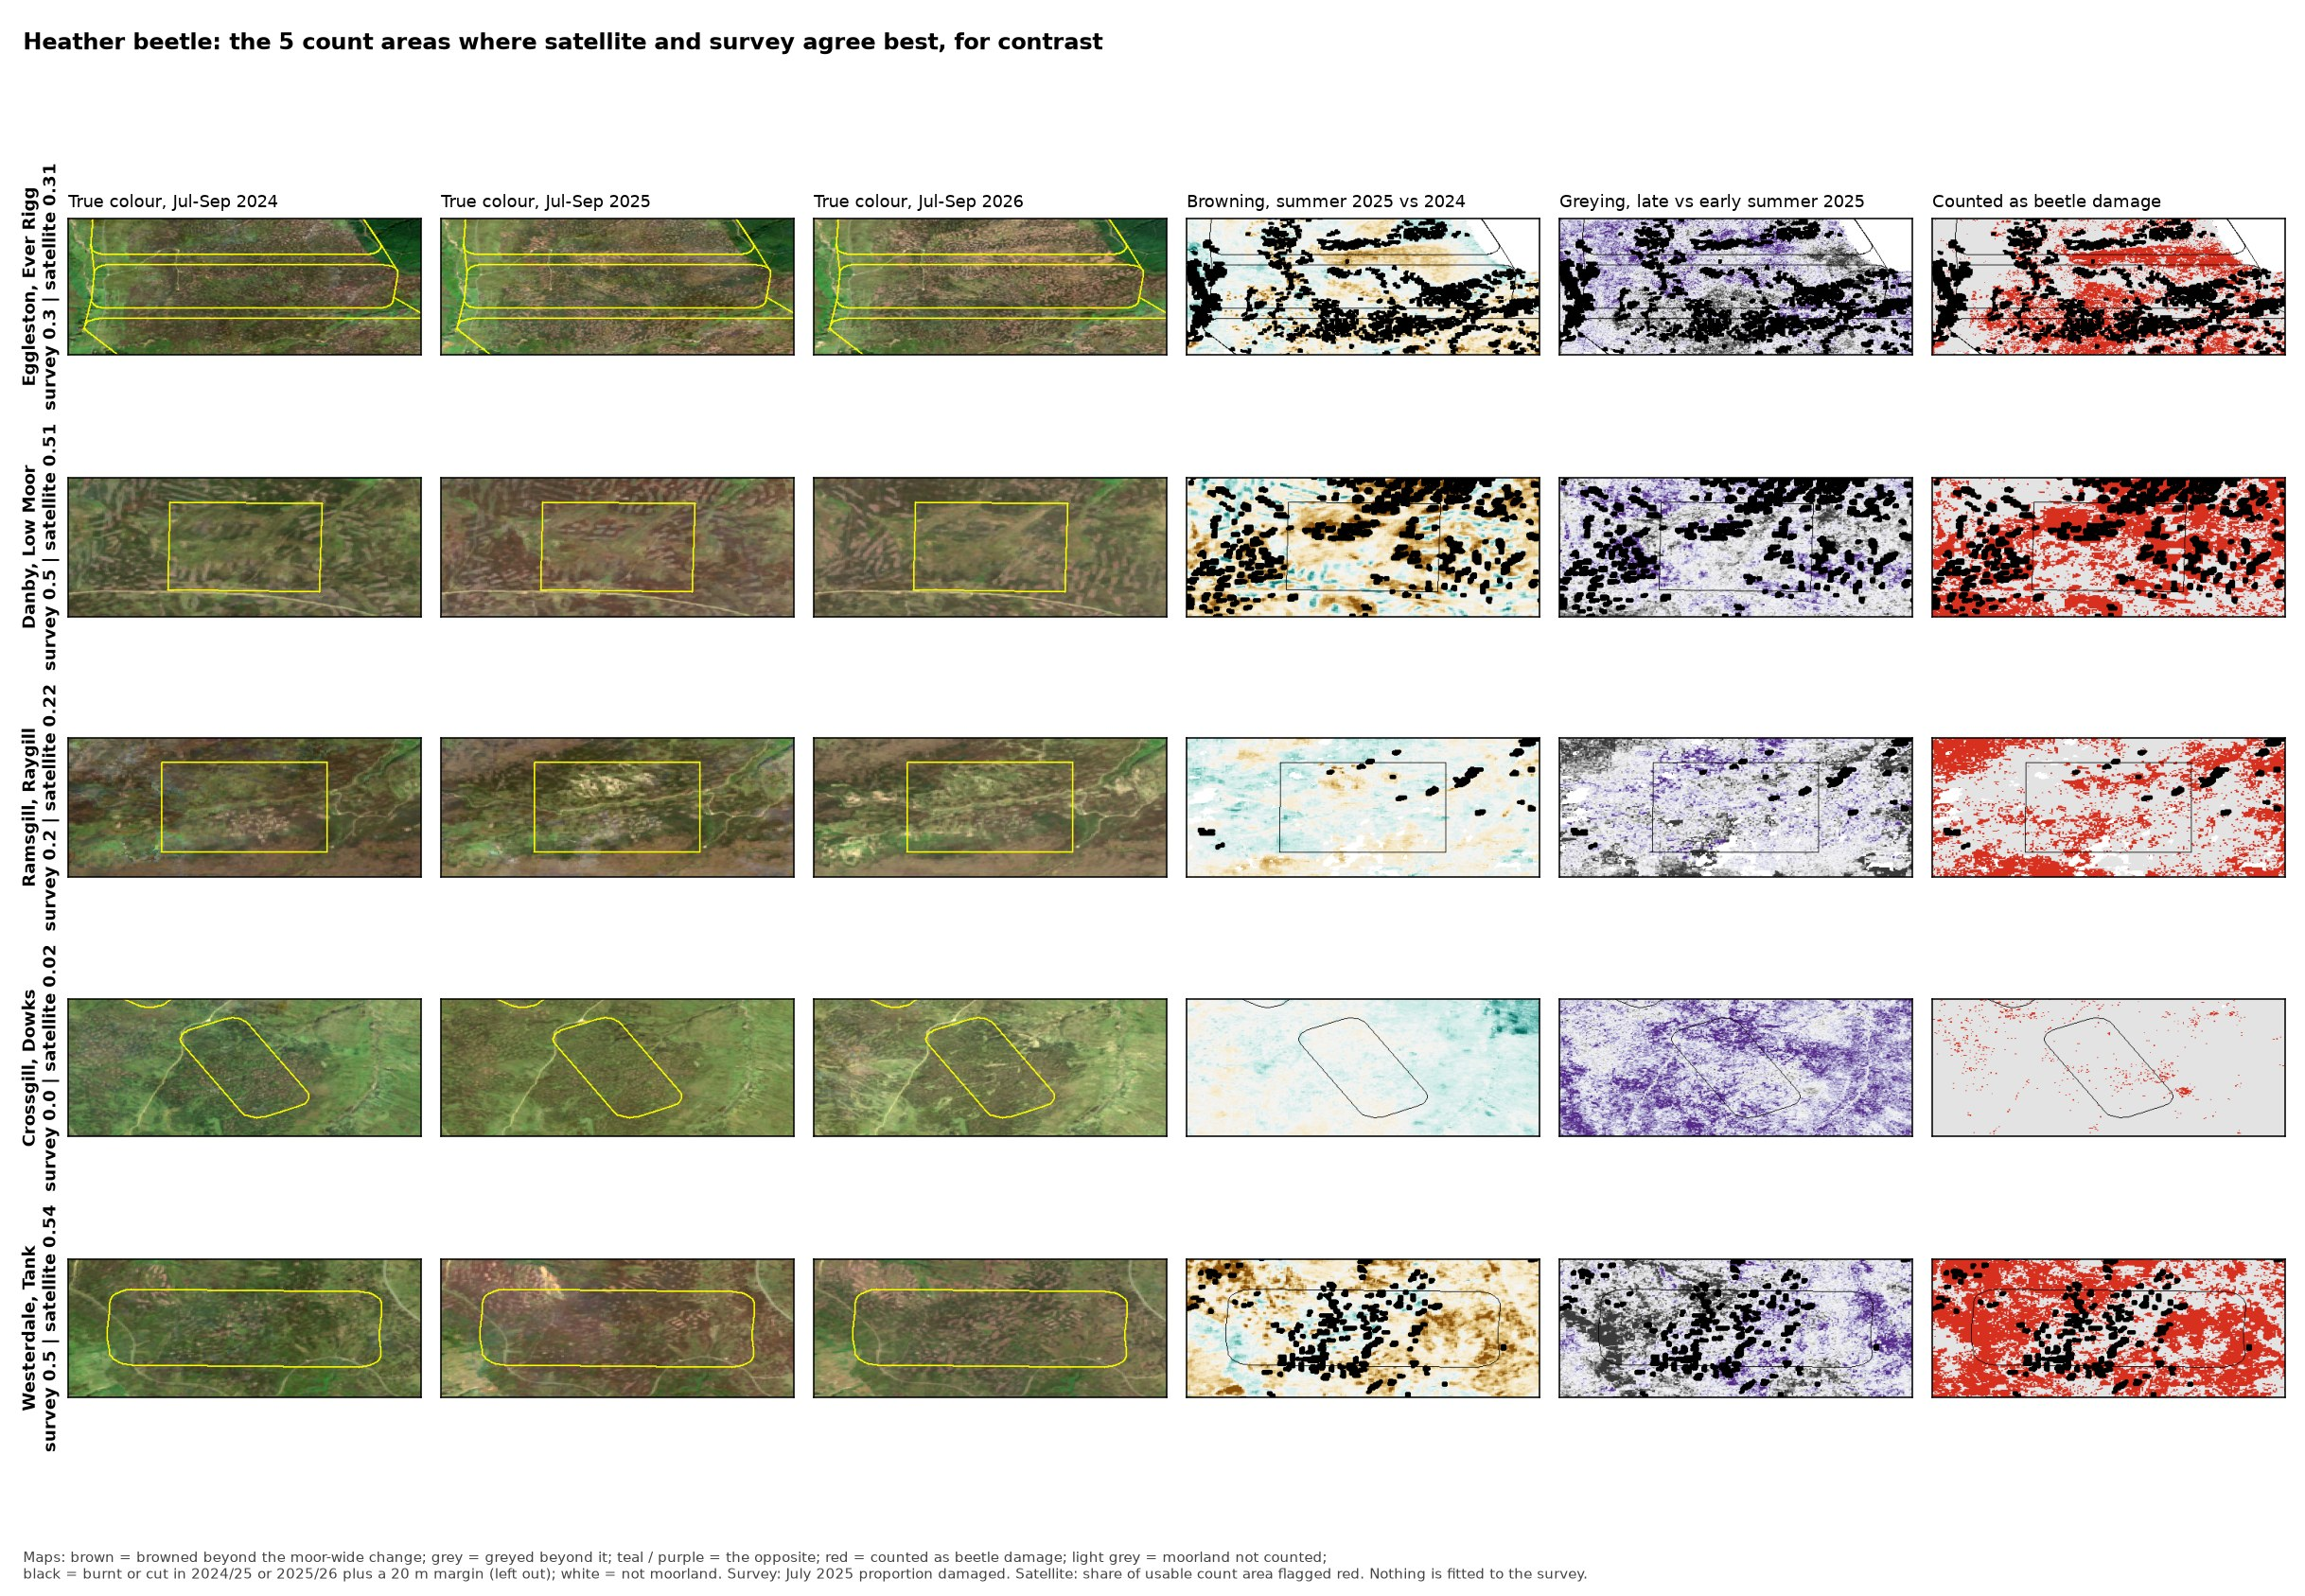
\includegraphics[width=\linewidth]{fig_evidence_agree.jpg}
\caption{The five count areas where the rule-based estimate and the survey agree best, for comparison with \figref{fig:evidence}.}\label{fig:evidence-agree}
\end{figure}

\clearpage
\section{Eggleston boundaries}\label{app:eggleston}

\begin{table}[H]
\centering
\caption{Eggleston and the North Pennines as count areas, as the strip between them, and as Eleanor's single block.}\label{tab:eggleston}
\small
\begin{tabular}{llrr}
\toprule
Scope & Boundary & Area (ha) & Mean \% a year \\
\midrule
Eggleston & count areas & 1,557 & 5.2 \\
Eggleston & strip between counts & 371 & 5.8 \\
Eggleston & count areas + strip (Eleanor's block) & 1,928 & 5.3 \\
North Pennines & count areas & 3,237 & 3.7 \\
North Pennines & strip between counts & 371 & 5.8 \\
North Pennines & count areas + strip (Eleanor's block) & 3,608 & 3.9 \\
\bottomrule
\end{tabular}

\end{table}

The strip between Eggleston's count areas is managed slightly more than the count areas themselves (5.8\% against 5.2\% a year), so including it would raise the North Pennines figure from 3.7\% to 3.9\%. None of the findings depends on the choice.

\section{Further imagery}\label{app:imagery}

\begin{figure}[H]
\centering
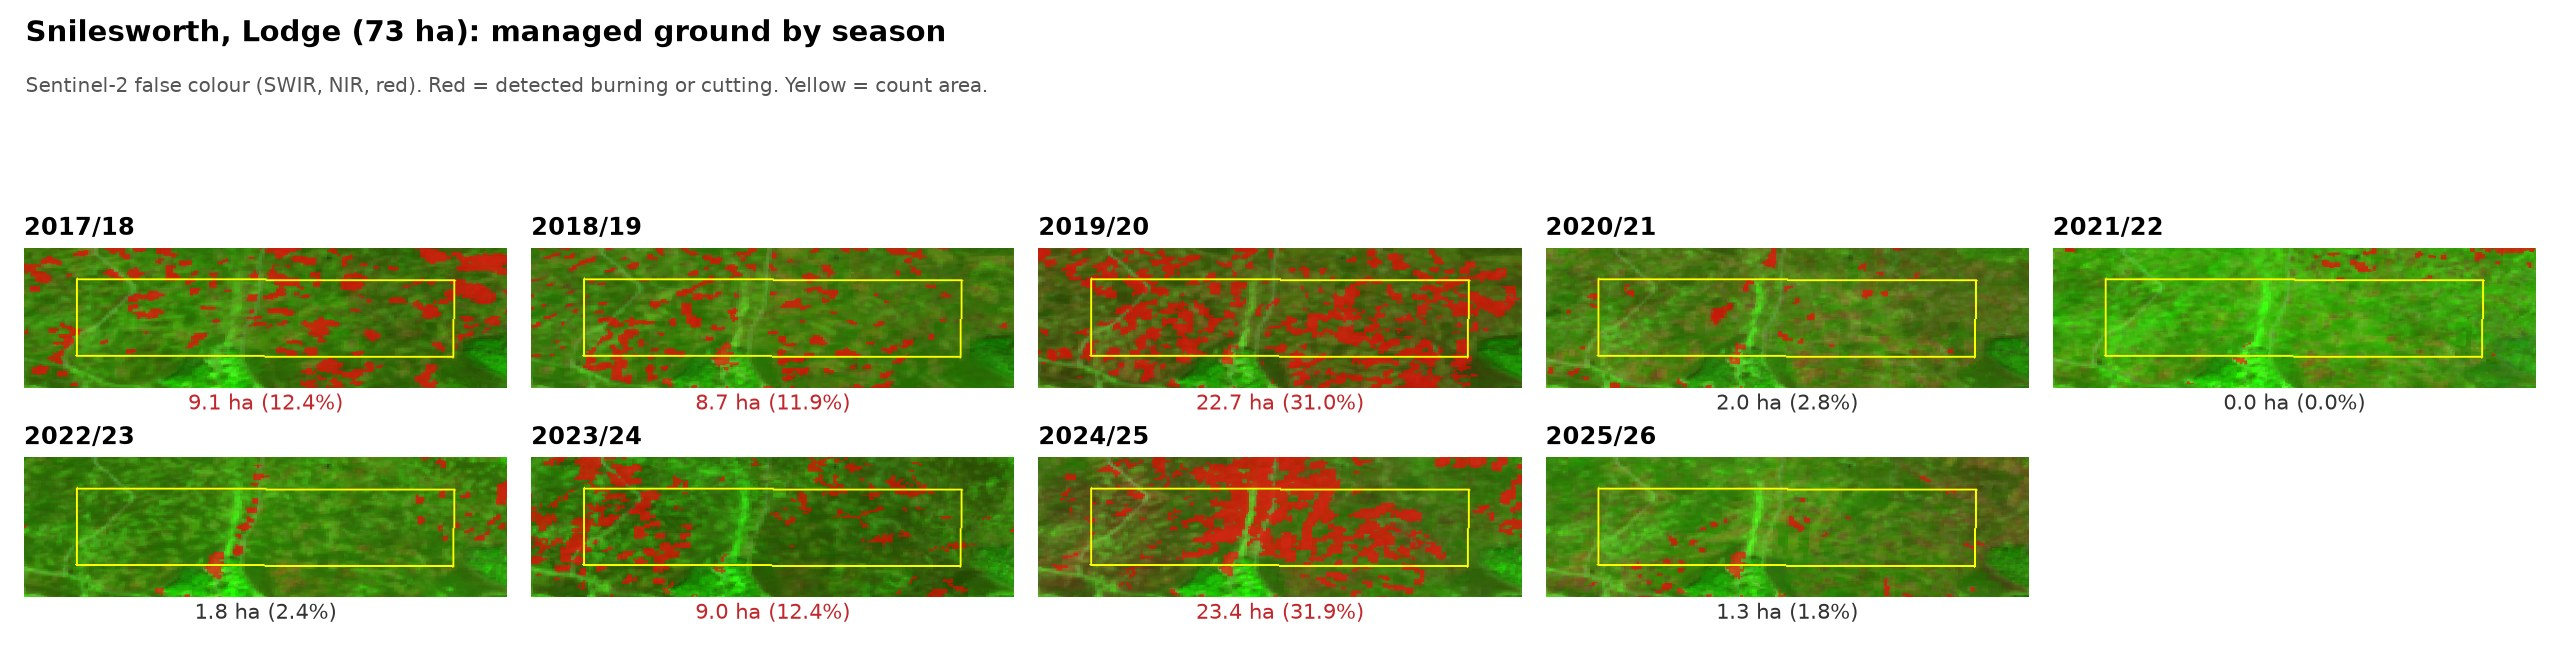
\includegraphics[width=\linewidth]{Snilesworth_Lodge.jpg}
\caption{Snilesworth, Lodge: the same sporadic pattern as Waskerley.}\label{fig:lodge}
\end{figure}

\begin{figure}[H]
\centering
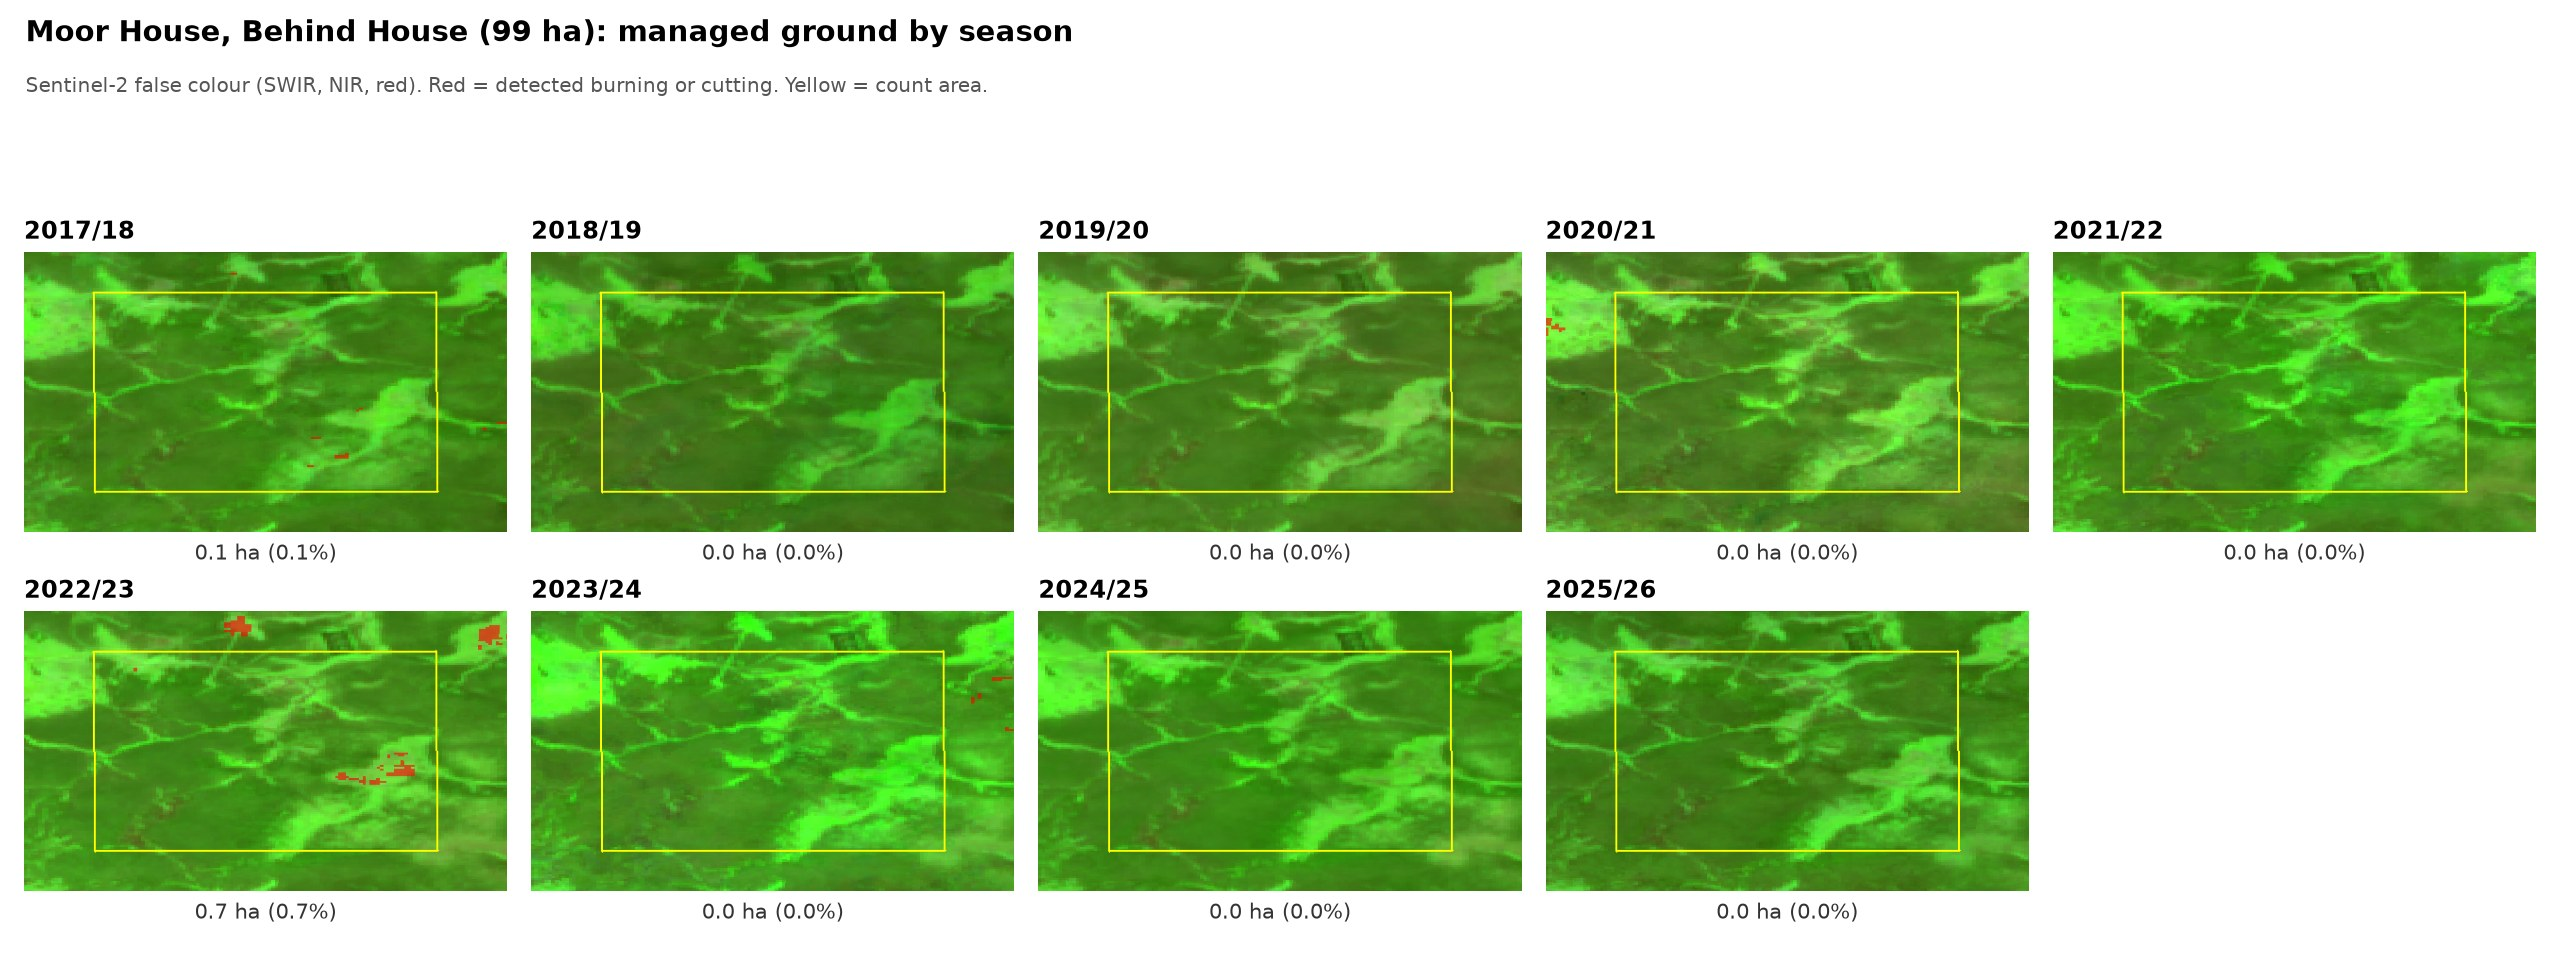
\includegraphics[width=\linewidth]{MoorHouse_BehindHouse.jpg}
\caption{Moor House, Behind House (National Nature Reserve): almost nothing detected in any season.}\label{fig:moorhouse}
\end{figure}

\begin{figure}[H]
\centering
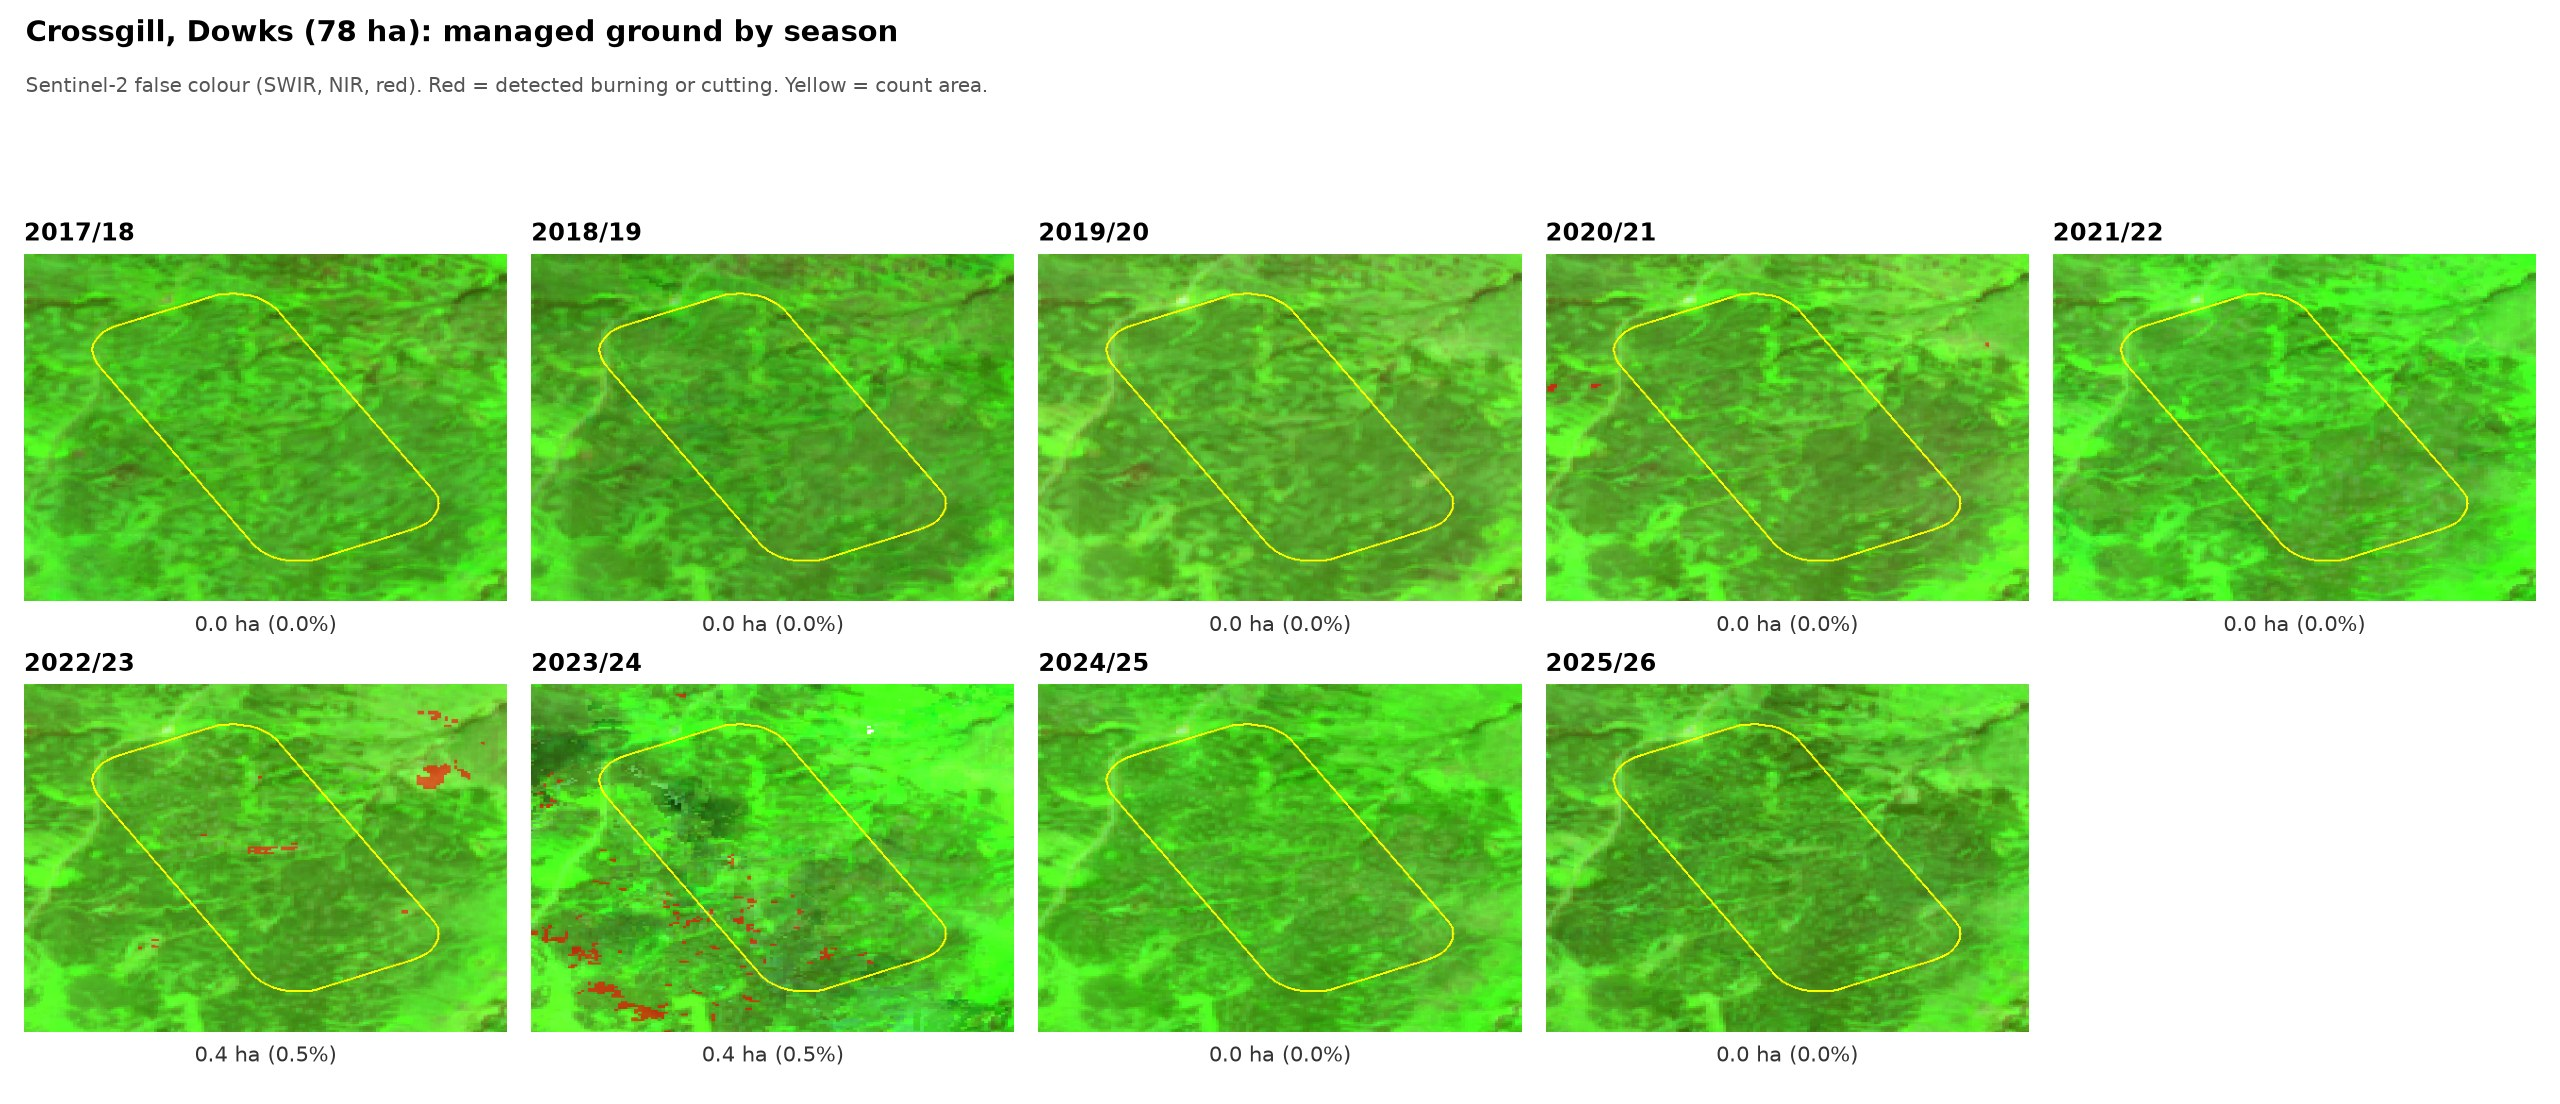
\includegraphics[width=\linewidth]{Crossgill_Dowks.jpg}
\caption{Crossgill, Dowks: at most 0.4~ha in any season. The small cuts PW describes are mostly below the 0.1~ha floor.}\label{fig:dowks}
\end{figure}

\begin{figure}[H]
\centering
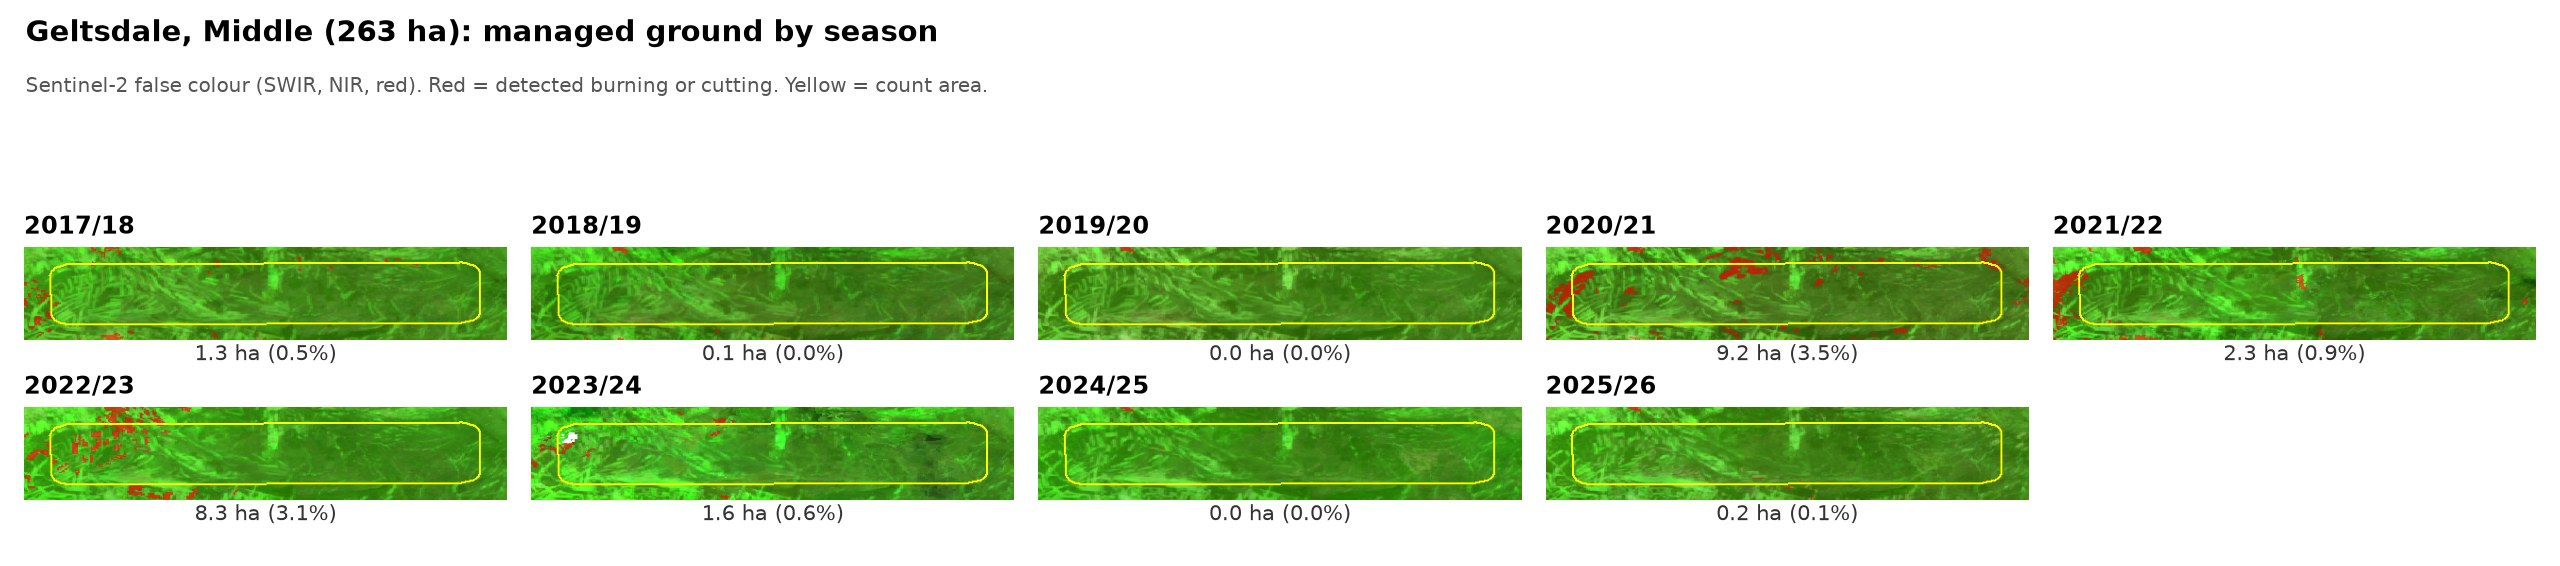
\includegraphics[width=\linewidth]{Geltsdale_Middle.jpg}
\caption{Geltsdale, Middle (RSPB reserve).}\label{fig:geltsdale}
\end{figure}

\FloatBarrier
\section{Data and code}\label{app:code}

\begin{table}[H]
\centering
\caption{Files behind this report.}\label{tab:files}
\footnotesize
\begin{tabularx}{\linewidth}{>{\raggedright\arraybackslash}p{0.40\linewidth}L}
\toprule
File & Contents \\
\midrule
\texttt{burn\_pipeline.py} & Detection pipeline (Earth Engine Python API) \\
\texttt{build\_count\_areas.py} & Names Eleanor's polygons from the transect file; splits Eggleston \\
\texttt{v5\_to\_v6\_changes.py} & Rebuilds version~1's boundaries; the one-change-at-a-time comparison \\
\texttt{beetle\_check.py}, \texttt{beetle\_rf.py}, \texttt{beetle\_model\_compare.py}, \texttt{beetle\_evidence.py} & Beetle damage: rule-based estimate, pixel sampling, gradient boosting and model comparison with leakage tests, image sheets \\
\texttt{report\_numbers.py}, \texttt{report/make\_figures.py} & Every number, figure and table in this report, from the outputs \\
\texttt{data/count\_areas\_v6.gpkg} & 28 count areas plus the Eggleston strip \\
\texttt{outputs/results\_by\_season.csv} & Results: 28 count areas by 9 seasons, threshold 0.17 \\
\texttt{outputs\_t013/}, \texttt{outputs\_t015/}, \texttt{outputs\_t019/}, \texttt{outputs\_no\_s2c/} & Sensitivity runs \\
\texttt{outputs\_abl\_*/}, \texttt{outputs/v5\_to\_v6/} & One-change-at-a-time runs and their summary \\
\texttt{outputs/beetle\_check/} & Beetle damage comparison \\
\bottomrule
\end{tabularx}
\end{table}

File and folder names use the internal numbering, in which this report is v6 and version~1 is v5.

\end{document}
